% Options for packages loaded elsewhere
\PassOptionsToPackage{unicode}{hyperref}
\PassOptionsToPackage{hyphens}{url}
%
\documentclass[
  12pt,
]{article}
\usepackage{lmodern}
\usepackage{amssymb,amsmath}
\usepackage{ifxetex,ifluatex}
\ifnum 0\ifxetex 1\fi\ifluatex 1\fi=0 % if pdftex
  \usepackage[T1]{fontenc}
  \usepackage[utf8]{inputenc}
  \usepackage{textcomp} % provide euro and other symbols
\else % if luatex or xetex
  \usepackage{unicode-math}
  \defaultfontfeatures{Scale=MatchLowercase}
  \defaultfontfeatures[\rmfamily]{Ligatures=TeX,Scale=1}
  \setmainfont[]{Times New Roman}
\fi
% Use upquote if available, for straight quotes in verbatim environments
\IfFileExists{upquote.sty}{\usepackage{upquote}}{}
\IfFileExists{microtype.sty}{% use microtype if available
  \usepackage[]{microtype}
  \UseMicrotypeSet[protrusion]{basicmath} % disable protrusion for tt fonts
}{}
\makeatletter
\@ifundefined{KOMAClassName}{% if non-KOMA class
  \IfFileExists{parskip.sty}{%
    \usepackage{parskip}
  }{% else
    \setlength{\parindent}{0pt}
    \setlength{\parskip}{6pt plus 2pt minus 1pt}}
}{% if KOMA class
  \KOMAoptions{parskip=half}}
\makeatother
\usepackage{xcolor}
\IfFileExists{xurl.sty}{\usepackage{xurl}}{} % add URL line breaks if available
\IfFileExists{bookmark.sty}{\usepackage{bookmark}}{\usepackage{hyperref}}
\hypersetup{
  pdftitle={Temporal, Spatial, and Regression Analyses of Lead Air Pollution Patterns and Sources in Pennsylvania},
  pdfauthor={Jack Alcorn, Max Hermanson, and Nancy Bao},
  hidelinks,
  pdfcreator={LaTeX via pandoc}}
\urlstyle{same} % disable monospaced font for URLs
\usepackage[margin=2.54cm]{geometry}
\usepackage{graphicx,grffile}
\makeatletter
\def\maxwidth{\ifdim\Gin@nat@width>\linewidth\linewidth\else\Gin@nat@width\fi}
\def\maxheight{\ifdim\Gin@nat@height>\textheight\textheight\else\Gin@nat@height\fi}
\makeatother
% Scale images if necessary, so that they will not overflow the page
% margins by default, and it is still possible to overwrite the defaults
% using explicit options in \includegraphics[width, height, ...]{}
\setkeys{Gin}{width=\maxwidth,height=\maxheight,keepaspectratio}
% Set default figure placement to htbp
\makeatletter
\def\fps@figure{htbp}
\makeatother
\setlength{\emergencystretch}{3em} % prevent overfull lines
\providecommand{\tightlist}{%
  \setlength{\itemsep}{0pt}\setlength{\parskip}{0pt}}
\setcounter{secnumdepth}{5}
\usepackage{booktabs}
\usepackage{longtable}
\usepackage{array}
\usepackage{multirow}
\usepackage{wrapfig}
\usepackage{float}
\usepackage{colortbl}
\usepackage{pdflscape}
\usepackage{tabu}
\usepackage{threeparttable}
\usepackage{threeparttablex}
\usepackage[normalem]{ulem}
\usepackage{makecell}
\usepackage{xcolor}

\title{Temporal, Spatial, and Regression Analyses of Lead Air Pollution
Patterns and Sources in Pennsylvania}
\usepackage{etoolbox}
\makeatletter
\providecommand{\subtitle}[1]{% add subtitle to \maketitle
  \apptocmd{\@title}{\par {\large #1 \par}}{}{}
}
\makeatother
\subtitle{\url{https://github.com/nyb5208/Alcorn_Bao_Hermanson_ENV_872_EDA_FinalProject.git}}
\author{Jack Alcorn, Max Hermanson, and Nancy Bao}
\date{}

\begin{document}
\maketitle

\newpage
\tableofcontents 
\newpage
\listoftables
\newpage
\listoffigures 
\newpage

\hypertarget{introduction}{%
\section{Introduction}\label{introduction}}

Lead is a heavy metal that is naturally found in the Earth's crust and
commonly used in many human products and industries (WHO, 2019).
However, its ubiquitous use has caused extensive environmental
contamination and public health concerns in many parts of the world (Ab
Latif Wani and Usmani, 2015). Main sources of lead contamination include
mining, smelting, manufacturing, recycling activities, leaded paint,
leaded gasoline, and leaded aviation fuel (US EPA, 2021a). Over three
quarters of global lead consumption is for the manufacturing of
lead-acid batteries for motor vehicles (WHO, 2019).

Once ingested, lead spreads through the blood into other parts of the
body. Depending on the level of exposure, lead can adversely affect the
nervous system, kidney function, immune system, reproductive and
developmental systems and the cardiovascular system (US EPA, 2020a). One
of the biggest health concerns of lead consumption is the neurological
effects on children. Children are particularly sensitive to lead
exposure and can have side effects such as behavioral problems, learning
disabilities, and lower IQ (Ab Latif Wani and Usmani, 2015).

Currently, the National Ambient Air Quality Standards (NAAQS) for lead
are 0.15 micrograms per cubic meter Pb in total suspended particles as a
3-month average (US EPA, 2021b). Air quality monitors are placed
throughout the United States in order to measure air lead levels. In our
project, we look at lead air quality monitors in the state of
Pennsylvania from 2010 to 2020.

\hypertarget{rationale}{%
\section{Rationale}\label{rationale}}

In this study, we were interested in evaluating lead air pollution in
Pennsylvania. In the 2019 United Health Foundation's annual American
Health Rankings report, Pennsylvania was rated 47th in the United States
for air quality (United Health Foundation, 2019). The metropolitan areas
around major Pennsylvania cities such as Pittsburgh, Philadelphia, and
Lancaster are currently ranked among the top 25 most polluted in the
country (American Lung Association, 2021). Pennsylvania's pollution
history is embedded in various industries such as agriculture,
manufacturing steel production, and coal mining and smelting (Stevens,
1955). The latter two have contributed to the current sources of lead
pollution in the air, soil, and water around the state (O'Shea et al.,
2020).

Other historical uses of lead in paints, gasoline, water pipes, and
batteries fueled the lead smelting industries in the state, especially
in major cities like Philadelphia (O'Shea et al., 2020). From a 2014
report from the Pennsylvania Department of Health, approximately 70\% of
homes in Pennsylvania were built prior to the leaded paint ban in 1978
(PA Department of Health, 2014); this has become a major source of human
lead exposure as homes begin aging and the leaded paint chips deposit
into the soil (O'Shea et al., 2020; PA Department of Health, 2014).
Current industrial emissions (e.g.~from smelters, airports, metal
processing facilities, incinerators) and lead from historical uses are
now found in soils and roadside dust that get resuspended into the
ambient air (US EPA, 2021a). Humans can be exposed to lead via
inhalation of resuspended dust and soil particles containing lead in the
air. Humans may also be exposed via ingestion of lead-contaminated
water, food, and dust (Pizzol and Andersen, 2010).

Considering Pennsylvania's industrial and historical uses of lead as
well as its current air quality status, we were interested in current
air lead pollution levels and lead exposure levels in Pennsylvania. We
decided to look at more recent temporal trends of air lead levels of the
EPA criteria pollutant, and chose a ten-year period from 2010 to 2020.
Furthermore, we were interested in identifying how air lead levels were
spatially associated with socioeconomic factors including income and
poverty at the county level. As lead is an EPA criteria pollutant, we
were also interested in exploring how sources of air lead
(e.g.~frequency of metal processing plants, airports, incinerators) may
be associated with lead exposure in children in Pennsylvania. These
analyses are summarized in the following research questions:

\#\#Research Questions:

\begin{enumerate}
\def\labelenumi{\arabic{enumi}.}
\item
  \textbf{\emph{How do air lead levels vary from 2010 to 2020 across the
  major metropolitan areas in Pennsylvania?}}
\item
  \textbf{\emph{What are the spatial associations between air lead
  levels and socioeconomic factors (ie. income and poverty) across
  counties in Pennsylvania?}}
\item
  \textbf{\emph{Is lead exposure (measured via blood lead levels) in
  children in Pennsylvania associated with air lead emission sources?}}
\end{enumerate}

\newpage

\hypertarget{dataset-information}{%
\section{Dataset Information}\label{dataset-information}}

\hypertarget{cdc-childhood-blood-lead-surveillance-data-blood-lead-levels-uxb5gdl-among-children-72-months-of-age-by-county-and-blood-lead-level-bll-group-2017-.csv}{%
\subsection{CDC Childhood Blood Lead Surveillance Data: Blood Lead
Levels (µg/dL) among Children \textless{} 72 Months of Age, by County
and Blood Lead Level (BLL) Group, 2017
(.csv)}\label{cdc-childhood-blood-lead-surveillance-data-blood-lead-levels-uxb5gdl-among-children-72-months-of-age-by-county-and-blood-lead-level-bll-group-2017-.csv}}

\begin{quote}
The CDC has a national surveillance system for assessing blood lead
levels (BLL). Data is collected from health-care provider reports to the
CDC on a variety of metrics, which include number of patients with BLL
greater than 5 µg/dL, and the average BLL of counties. The CDC notes
these data may be biased by the fact that those who are tested for
elevated BLL are typically tested because they predisposed to higher
levels due to certain criteria.
\end{quote}

\hypertarget{federal-aviation-administration-airport-data-shapefile}{%
\subsection{Federal Aviation Administration Airport Data
(shapefile)}\label{federal-aviation-administration-airport-data-shapefile}}

\begin{quote}
These data are collected by the FAA through legally-required reporting
by existing airports. This dataset is updated regularly, and the data
used in our research project was from April, 2021. Notable attributes
included for each airport were geographic coordinates, status active,
airport purpose, and type of aircraft used at the airport.
\end{quote}

\hypertarget{pennsylvania-department-of-environmental-protection-dep-database-on-mineral-preparation-plants-and-incinerators-shapefile}{%
\subsection{Pennsylvania Department of Environmental Protection (DEP)
Database on Mineral Preparation Plants and Incinerators
(shapefile)}\label{pennsylvania-department-of-environmental-protection-dep-database-on-mineral-preparation-plants-and-incinerators-shapefile}}

\begin{quote}
A mineral preparation plant is a site at which extracted minerals are
processed in order to separate and purify elements and compounds of
interest. These processes typically require heating the minerals to very
high temperatures, which can release lead particulates into the air. The
DEP keeps track of the location, owner, site status, and primary
facility type of these plants. Data used in this study were dated to
April of 2021.
\end{quote}

\begin{quote}
Detailed and regular incinerator data is also maintained by the DEP
(last updated in April 2021). Incinerators combust waste products, which
emits particulate matter whose composition depends upon the type of
waste being burned. Incinerators are used for a variety of materials,
including garbage, industrial scrap products, hospital waste, and dead
organisms or cadavers. Filters were applied to select only
industrial-waste-related incinerators that might possess lead
particulates.
\end{quote}

\hypertarget{us-census-metropolitan-and-micropolitan-statistical-area-population-estimates-and-estimated-components-of-change-april-1-2010-to-july-1-2019}{%
\subsection{US Census Metropolitan and Micropolitan Statistical Area
Population Estimates and Estimated Components of Change: April 1, 2010
to July 1,
2019}\label{us-census-metropolitan-and-micropolitan-statistical-area-population-estimates-and-estimated-components-of-change-april-1-2010-to-july-1-2019}}

\begin{quote}
Metropolitan and Micropolitan Statistical Area Population Estimates and
Estimated Components of Change were collected by the US Census in 2019
across the United States. Estimates for total population size, numeric
change in total population, births, deaths, natural increase periods
defined by births minus deaths, net domestic migration, net
international migration, net migration periods, and residuals from 2011
to 2019 were based on population size data from the 2010 US Census (US
Census Bureau, 2020a). The dataset also contains the population size
reported in the 2010 US Census as the variable, CENSUS2010POP. The
following dataset contained the following identifier variables for the
metropolitan and micropolitan statistical areas in the United States:
name of the statistical area (NAME), the 5-digit core statistical based
area (CBSA) code, and the legal statistical area description (LSAD) (US
Census Bureau, 2020b). For this study, only the following variables were
used: CBSA, NAME, LSAD, and CENSUS2010POP.
\end{quote}

\hypertarget{us-epa-daily-air-lead-data-2010-2020}{%
\subsection{US EPA Daily Air Lead Data
2010-2020}\label{us-epa-daily-air-lead-data-2010-2020}}

The daily air lead levels data were collected from all outdoor
monitoring sites from the US EPA Air Quality System Data Mart. Data for
each year were individually downloaded from the US EPA Outdoor Air
Quality Database. The daily air lead levels were taken from 24-hr
average lead level observations measured in ug/m\^{}3 and recorded by
the air quality System (AQS) (About Air Data Reports, 2021). The data
included the following variables: date of air lead measurement, source
of data, the daily mean lead concentration ug/m\^{}3, daily observation
count, and data completion percentage, based on the site monitoring
frequency and schedule (About Air Data Reports, 2021).

The following site identifier variables were also included in the
datasets: parameter occurrence code (POC), which specifies the monitor
number that collected the data, 5-digit AQS parameter code, site name,
2-digit state federal information processing system (FIPS) code, state
name, the 3-digit county FIPS code, county name, site ID (composed of
the state FIPs code, county FIPS code, and 4-character AQS code), core
statistical based area (CBSA) name and code for the metropolitan area
designated to the monitoring site, and the site latitude and longitude
coordinates (About Air Data Reports, 2021).

\hypertarget{cdc-social-vulnerability-data-2010-and-2018}{%
\subsection{CDC Social Vulnerability Data (2010 and
2018)}\label{cdc-social-vulnerability-data-2010-and-2018}}

Social Vulnerability data was collected over five year time periods in
the state of Pennsylvania using the American Community Survey. For the
2010 data, data was collected from 2006-2010 and the 2018 data was
collected from the years 2014-2018. Questions involved in the survey
covered vulnerability topics such as socioeconomic status, household
composition and disability, minority status and language, and housing
type and transportation. The data set included over one hundred
variables. The variables used in the following analysis include county
name, per capita income (E\_PCI), and percentage of persons below
poverty estimate (EP\_POV). \newpage \# Methods \#\# Question 1: How do
air lead levels vary from 2010 to 2020 across the major metropolitan
areas in Pennsylvania? \#\#\# Data Wrangling US EPA daily mean air lead
concentration data for each year from 2010 to 2020 were individually
read into RStudio as separate dataframes and combined into one dataframe
for all daily mean air lead levels from 2010 to 2020, using the rbind()
function. The combined data frame was further processed with a pipe that
selected for the date lead levels were collected, the monitoring site
ID, the site name, the CBSA name and code identifiers, state name,
county name and county FIPS code; a new variable for month, year, and
date formatted as month-year were created using the mutate() function.

Air lead levels from 2010 to 2020 were assessed across Pennsylvania by
metropolitan statistical areas. The top five most populous metropolitan
areas were the focus of this portion of the study. The reason is that
these areas were assumed to have historically higher industrial
emissions and more sources of lead associated with legacy paint and
gasoline, and sources from aviation fuel from airports (US EPA, 2020a).
Furthermore, the Air Quality System only collected lead concentration
measurements for 15 counties in Pennsylvania across this period, and so
we were limited to analyses at the metropolitan area level rather than
at the county level.

US Census data for Metropolitan and Micropolitan Statistical Area
Population Estimates and Estimated Components of Change: April 1, 2010
to July 1, 2019 were read in as a dataframe and processed with a
pipeline that selected for metropolitan area data by the 5-digit CBSA
code, names of the metropolitan areas that overlapped with the US EPA
daily mean lead concentration dataset, as well as the 2010 US Census
reported population size. The top five metropolitan areas by population
size (1= most populous) in Pennsylvania were identified as (1)
Philadelphia-Camden-Wilmington, PA-NJ-DE-MD, (2)Pittsburgh, PA,
(3)Allentown-Bethlehem-Easton, PA-NJ,
(4)Scranton--Wilkes-Barre--Hazleton, PA, (5)Lancaster, PA.

The processed, combined 2010-2020 US EPA daily mean air lead
concentrations dataframe were filtered by the unique CBSA codes for each
metropolitan area and individual data frames were created for each
metropolitan area which contained their respective date and lead
concentration measurements.

\hypertarget{exploratory-analysis}{%
\subsubsection{Exploratory Analysis}\label{exploratory-analysis}}

A new variable was created using the mutate() function to summarize and
calculate the monthly mean air lead levels for each metropolitan area
dataframe. Monthly mean air lead levels for all metropolitan areas were
calculated from 2010 to 2020. Line plots were generated for the monthly
mean air lead levels for each metropolitan area to assess the trends in
air lead levels between 2010 to 2020. The monthly air lead levels were
graphed in three-month intervals in each metropolitan area and were
compared to the primary and secondary EPA 3-month rolling average NAAQS
for lead, 0.15ug/m\^{}3.

\hypertarget{data-analysis}{%
\subsubsection{Data Analysis}\label{data-analysis}}

The daily mean air lead data for each metropolitan area data frame
contained missing air lead concentration measurements for certain days
and a linear interpolation was applied to the daily mean air lead levels
for each metropolitan area. Spline interpolations were not used as data
did not follow a quadratic or higher-order polynomial trend. Linear
interpolation was used over piecewise interpolation because our study
was interested in the change in air lead levels over a continuous
ten-year period of time from 2010 to 2020. The linearly interpolated
daily mean air lead levels for each metropolitan area were combined into
one dataframe. Following linear interpolation of the daily mean air lead
levels for each metropolitan area dataframe, the data frames were
converted into time series objects for daily observations and monthly
observations. Seasonality was not observed for the interpolated daily
mean air lead levels for the metropolitan areas. Nonseasonal
Mann-Kendall trend tests were conducted on the daily and monthly time
series objects for mean air lead levels for each of the five
metropolitan areas.

\hypertarget{question-2-what-are-the-spatial-associations-between-air-lead-levels-and-socioeconomic-factors-ie.-income-and-poverty-across-counties-in-pennsylvania}{%
\subsection{Question 2: What are the spatial associations between air
lead levels and socioeconomic factors (ie. income and poverty) across
counties in
Pennsylvania?}\label{question-2-what-are-the-spatial-associations-between-air-lead-levels-and-socioeconomic-factors-ie.-income-and-poverty-across-counties-in-pennsylvania}}

\hypertarget{data-wrangling}{%
\subsubsection{Data Wrangling}\label{data-wrangling}}

Data wrangling began with grouping EPA air lead concentration data by
county, latitude and longitude for the years of 2010, 2015, and 2020
using the group\_by() function. County mean and maximum lead
concentrations for 2010, 2015, and 2020 were computed by averaging all
county daily mean lead concentrations and selecting the maximum county
daily mean lead concentration through the summarize () function. These
data sets were then converted into spatial features st\_as\_sf ()
function and using NAD 83 as a coordinate reference system. EPA mean and
maximum air lead concentration values were then joined with a
Pennsylvania county shape file, county per capita income estimates and
percentage of people in poverty estimates using the left\_join ()
function. These data frames were joined by the county column. We also
looked at lead concentrations that exceeded air quality standards of .15
micrograms per cubic meter for 2010, 2015, and 2020. To obtain max lead
concentrations over .15 micrograms per cubic meter, values that exceeded
this limit in the EPA air lead concentration were filtered out of the
EPA air lead concentration data using the filter() function.

\hypertarget{exploratory-analysis-1}{%
\subsubsection{Exploratory Analysis}\label{exploratory-analysis-1}}

Data exploration used graphs to visually analyze lead concentration for
2010, 2015 and 2020. Different data visualization techniques were
experimented with to determine what best represented the data and made
the graphs visually appealing. Mean population for each county was also
considered as a variable for spatial associations of high lead
concentrations but this did not prove to be useful when graphed. This
variable was taken out of the analysis.

\hypertarget{data-analysis-1}{%
\subsubsection{Data Analysis}\label{data-analysis-1}}

Analysis consisted of overlaying per capita income and percentage of
people in poverty estimates on top of mean and max air lead
concentration values. In the end, maps were created for lead
concentration levels paired with either per capita income or percentage
of persons below poverty for all years. These were visually compared to
each other to determine trends in the past to years and if the variables
used showed spatial association. Maps were also created for the max lead
concentration levels that were above .15 micrograms per cubic meter.
These were used to analyze differences between all three years.

\hypertarget{question-3-is-lead-exposure-measured-via-blood-lead-levels-in-children-in-pennsylvania-associated-with-air-lead-emission-sources}{%
\subsection{Question 3: Is lead exposure (measured via blood lead
levels) in children in Pennsylvania associated with air lead emission
sources?}\label{question-3-is-lead-exposure-measured-via-blood-lead-levels-in-children-in-pennsylvania-associated-with-air-lead-emission-sources}}

\hypertarget{data-wrangling-1}{%
\subsubsection{Data Wrangling}\label{data-wrangling-1}}

\begin{enumerate}
\def\labelenumi{\arabic{enumi}.}
\tightlist
\item
  Matching coordinates with counties Shape files for specific metal
  processing plants, incinerators, and airports were individually read
  as separate dataframes and converted to `sf' dataframes within R, and
  the `st\_intersects' function was used in conjunction with U.S. 2010
  census data to identify in which county each of these features were
  located.
\end{enumerate}

Specific types of metal processing plants, incinerators, and airports
were filtered out using the filter() function for a variety of criteria
specified in the Dataset Description section of this document.

\begin{enumerate}
\def\labelenumi{\arabic{enumi}.}
\setcounter{enumi}{1}
\item
  Combining datasets into one (converted column classes, renamed
  columns) It was important to compile attribute information for each
  county into a single dataframe so that a regression could be run upon
  each county observation. In order to combine separate dataframes for
  the aforementioned shapefiles, class differences and syntax
  differences between the columns and their values were resolved. Common
  changes that had to occur were getting rid of leading zeros (001
  vs.~1) and renaming the county code columns for each attribute to
  ``COUNTYFP10'' (later on, Jack's county per capita income and county
  poverty sf dataframes were merged into this dataframe to include more
  variables into the model).
\item
  Cleaning and prepping data Data was cleaned and prepped for
  transformations: replaced NA's with zeros for the plant/airport data
  and added small integer values to all data in order to log transform
  variables with values of zero.
\end{enumerate}

\hypertarget{exploratory-analysis-2}{%
\subsubsection{Exploratory Analysis}\label{exploratory-analysis-2}}

\begin{enumerate}
\def\labelenumi{\arabic{enumi}.}
\tightlist
\item
  Examined distribution of variables and transformed where necessary The
  variables' distributions were examined, and individual scatter plots
  for each explanatory variable (EV) were created against the response
  variables to check for linearity. Based on these results, the metal
  processing plant data (METAL) and incinerator data (INCINERATE) were
  logged, and the county poverty data (POV) were squared to be a
  quadratic term. Residuals v Fitted graphs of these showed better fits.
  \#\#\# Data Analysis
\item
  Tested assumptions An ordinary least squares (OLS) multilinear
  regression was carried out. The following assumptions were tested for:
  linearity, homoscedasticity, multicollinearity, and normality.
\end{enumerate}

Based on the residuals vs fitted plot, the final model is non-linear. It
possesses an upward-cone shape and the red trend line sharply trails off
at higher fitted values. The final model appears to be heteroskedastic
based on its scale-location graph, which sharply deviates from zero at
higher fitted values. This model does not meet the homoskedasticity
assumption. Multicollinearity was examined using the vif() function,
which conducts a Variance Inflation Factor between explanatory
variables. Values above two are considered moderately correlated, but
given how close two most of them were, mean-centering was not performed.
This model met the normality assumption based on the Normal Q-Q plot.
\newpage

\newpage

\hypertarget{results}{%
\section{Results}\label{results}}

\hypertarget{question-1-how-do-air-lead-levels-vary-from-2010-to-2020-across-the-major-metropolitan-areas-in-pennsylvania}{%
\subsection{Question 1: How do air lead levels vary from 2010 to 2020
across the major metropolitan areas in
Pennsylvania?}\label{question-1-how-do-air-lead-levels-vary-from-2010-to-2020-across-the-major-metropolitan-areas-in-pennsylvania}}

From the lineplot of the linearly interpolated daily mean air lead
levels for the five metropolitan areas, we see that mean daily lead
levels appear to be decreasing from 2010 to 2020. It is important to
note that the time intervals vary between the metropolitan areas for
mean daily air lead measurements. Mean daily air lead levels were
measured from 2010 to 2020 for the Pittsburgh, PA and the
Philadelphia-Camden-Wilmington, PA-NJ-DE-MD metropolitan areas. Mean
daily air lead levels were measured from 2012 to 2020 for the Lancaster,
PA and the Allentown-Bethlehem-Easton, PA-NJ metropolitan areas. The
mean daily air lead levels were measured from 2010 to 2018 for the
Scranton--Wilkes-Barre--Hazleton, PA metropolitan areas.

To further assess the trends, the non-seasonal Mann-Kendall trend tests
for the daily time series objects found that four of the five most
populous metropolitan followed significant, monotonic trends for daily
and monthly mean air lead levels. The Mann-Kendall trend test for the
daily time series found significant (p\textless0.05) downward monotonic
trends for mean daily air lead levels the following metropolitan areas:
Philadelphia-Camden-Wilmington, PA-NJ-DE-MD (tau = -0.168,
p-value=\textless{} 2.22e-16), Pittsburgh, PA (tau = -0.276,
p-value=\textless{} 2.22e-16), Allentown-Bethlehem-Easton, PA-NJ (tau=
-0.257 , p-value=\textless{} 2.22e-16 ),
Scranton--Wilkes-Barre--Hazleton, PA (tau=-0.53, , p-value=\textless{}
2.22e-16). Lancaster, PA had a downward, non-monotonic trend
(p\textgreater0.05) for daily mean air lead levels (tau=-0.0181, p-value
=0.145). The nonseasonal Mann-Kendall trend tests for the monthly time
series objects found significant (p\textless0.05) downward monotonic
trends for the following metropolitan areas:
Philadelphia-Camden-Wilmington, PA-NJ-DE-MD (tau=-0.711 ,
p-value\textless2.22e-16 ), Pittsburgh, PA (tau=-0.755,
p-value\textless2.22e-16 ), Allentown-Bethlehem-Easton, PA-NJ (tau=
-0.378 , p-value= 1.78e-08 ), and Scranton--Wilkes-Barre--Hazleton, PA
(tau=-0.593 , p-value\textless2.22e-16 ). There was a non-monotonic
(p-value\textgreater0.05) downward trend observed for monthly mean air
lead levels in Lancaster, PA (tau= -0.0055, p-value = 0.934).

\begin{figure}

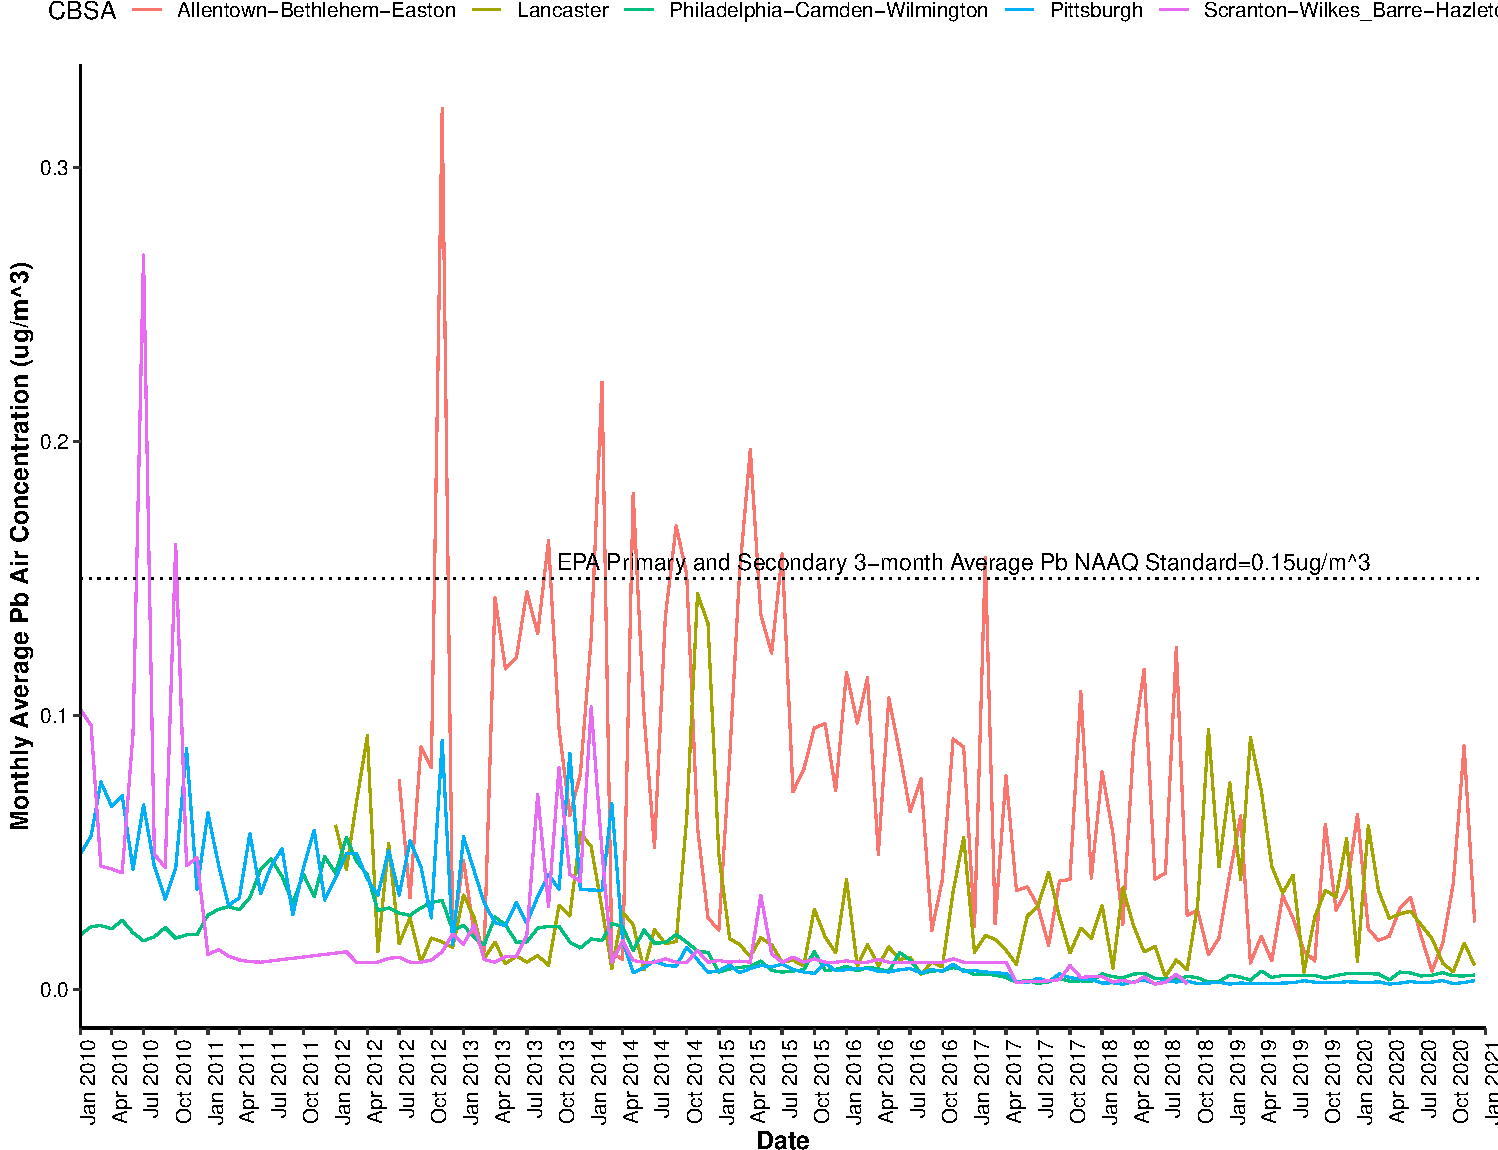
\includegraphics{Alcorn_Bao_Hermanson_ENV872_Project_files/figure-latex/time-series-visuals-1} \hfill{}

\caption{Monthly Average Pb Air Concentrations from 2010 to 2020 in PA Metro Areas}\label{fig:time-series-visuals}
\end{figure}

\begin{verbatim}
## [1] "Date"
\end{verbatim}

\begin{figure}

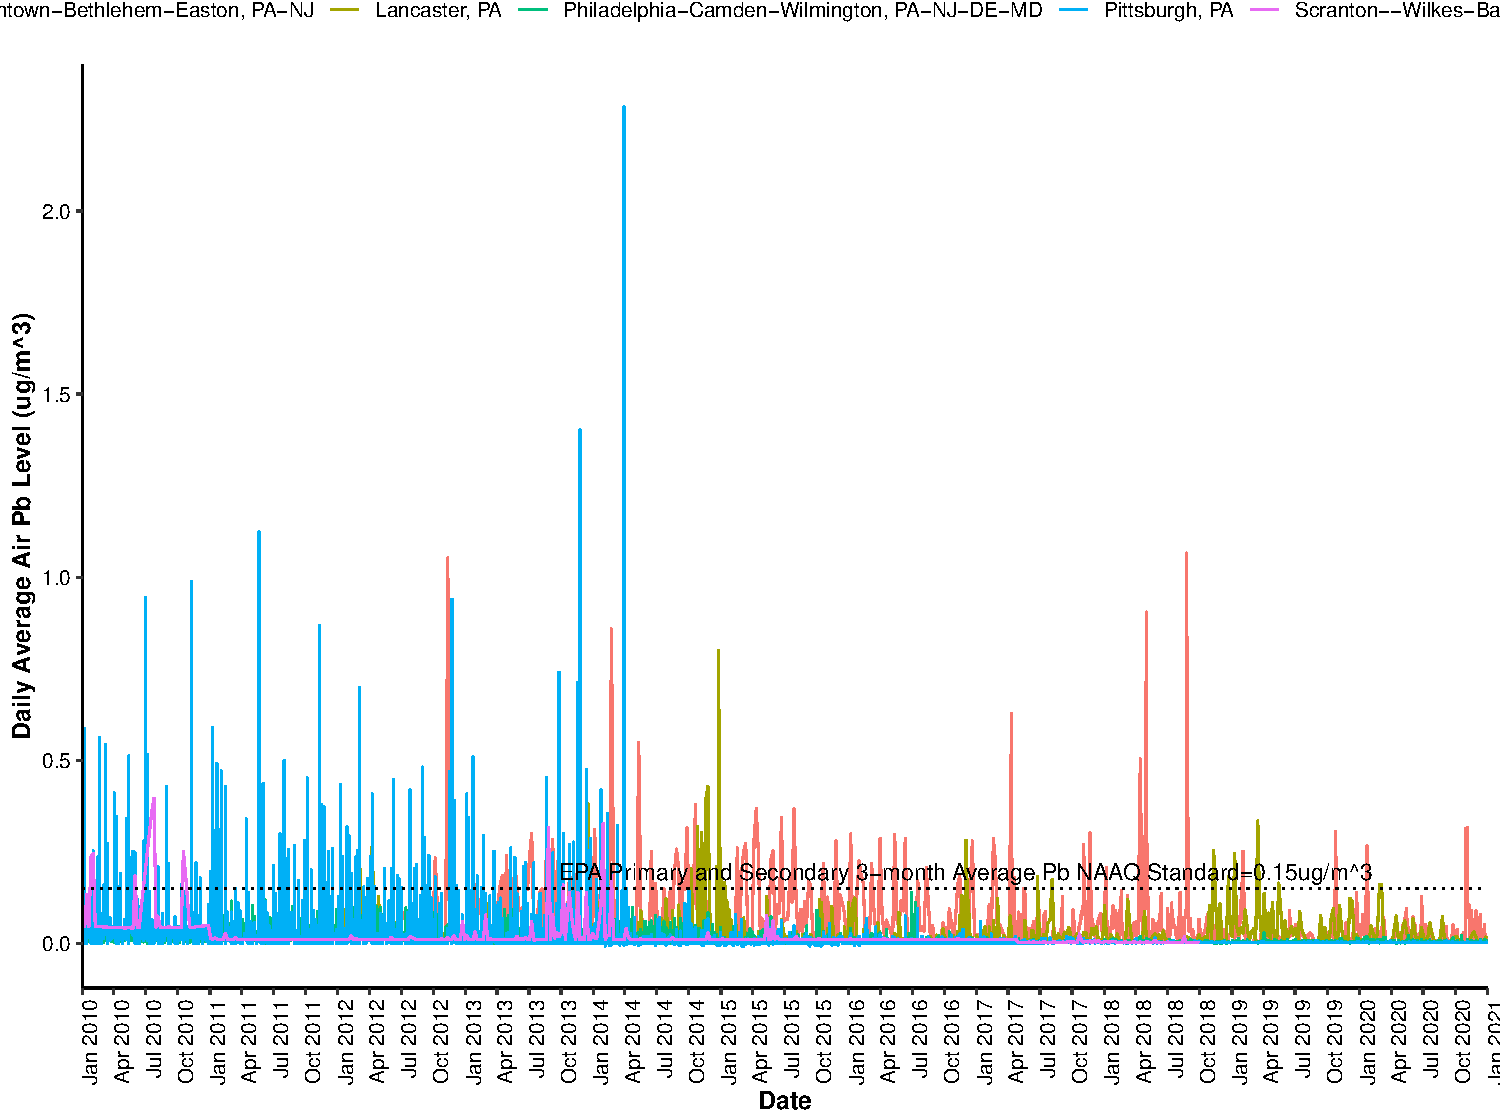
\includegraphics{Alcorn_Bao_Hermanson_ENV872_Project_files/figure-latex/linear-interp-visual-1} \hfill{}

\caption{Daily average air Pb levels from 2010 to 2020 in the five most populous metropolitan areas in PA}\label{fig:linear-interp-visual}
\end{figure}

\hypertarget{question-2-what-are-the-spatial-associations-between-air-lead-levels-and-socioeconomic-factors-ie.-income-and-poverty-across-counties-in-pennsylvania-1}{%
\subsection{Question 2: What are the spatial associations between air
lead levels and socioeconomic factors (ie. income and poverty) across
counties in
Pennsylvania?}\label{question-2-what-are-the-spatial-associations-between-air-lead-levels-and-socioeconomic-factors-ie.-income-and-poverty-across-counties-in-pennsylvania-1}}

The spatial analysis confirmed that mean lead concentration levels have
gone down from 2010 to 2020. The highest mean concentration levels for
2010 was .15 ug/m\^{}3 compared to .1 ug/m\^{}3 for 2015 and .03
ug/m\^{}3 for 2020. The graphs also showed where high lead
concentrations resided in the state of Pennsylvania. Counties that had
the highest concentrations were Lancaster, Berks, Lehigh, Beaver,
Allegheny, and Indiana. These are areas that have medium levels of
people below poverty and tend to have lower per capita income levels
compared with the rest of the state. When looking at the amount of
maximum lead concentration levels that were above the air quality
standard of .15 ug/m\^{}3, 2010 had 7 locations that exceeded this
limit. Berks and Beaver each had two areas with readings above .9
ug/m\^{}3. For 2015 and 2020, there were only three locations (for each
year) that exceeded the air quality standard limit. Beaver county had
zero areas during these years and Berks county reduced to only one
reading at approximately .24 ug/m\^{}3. This spatial analysis assists
with the time series analysis done in the section above. Moving forward,
doing an analysis at a smaller scale would provide improved results.
Future analysis could look at counties, such as Berks and Beaver, and
perform analysis at the zip code level.

\begin{verbatim}
## [1] 0.02118966 0.17580357
\end{verbatim}

\begin{verbatim}
## Reading layer `cb_2018_us_county_20m' from data source `/Users/mothership/Desktop/EDA_21/Alcorn_Bao_Hermanson_ENV_872_EDA_FinalProject/Data/Spatial/cb_2018_us_county_20m.shp' using driver `ESRI Shapefile'
## Simple feature collection with 3220 features and 9 fields
## Geometry type: MULTIPOLYGON
## Dimension:     XY
## Bounding box:  xmin: -179.1743 ymin: 17.91377 xmax: 179.7739 ymax: 71.35256
## Geodetic CRS:  NAD83
\end{verbatim}

\begin{verbatim}
## [1] 15691.33 40670.86
\end{verbatim}

\begin{figure}

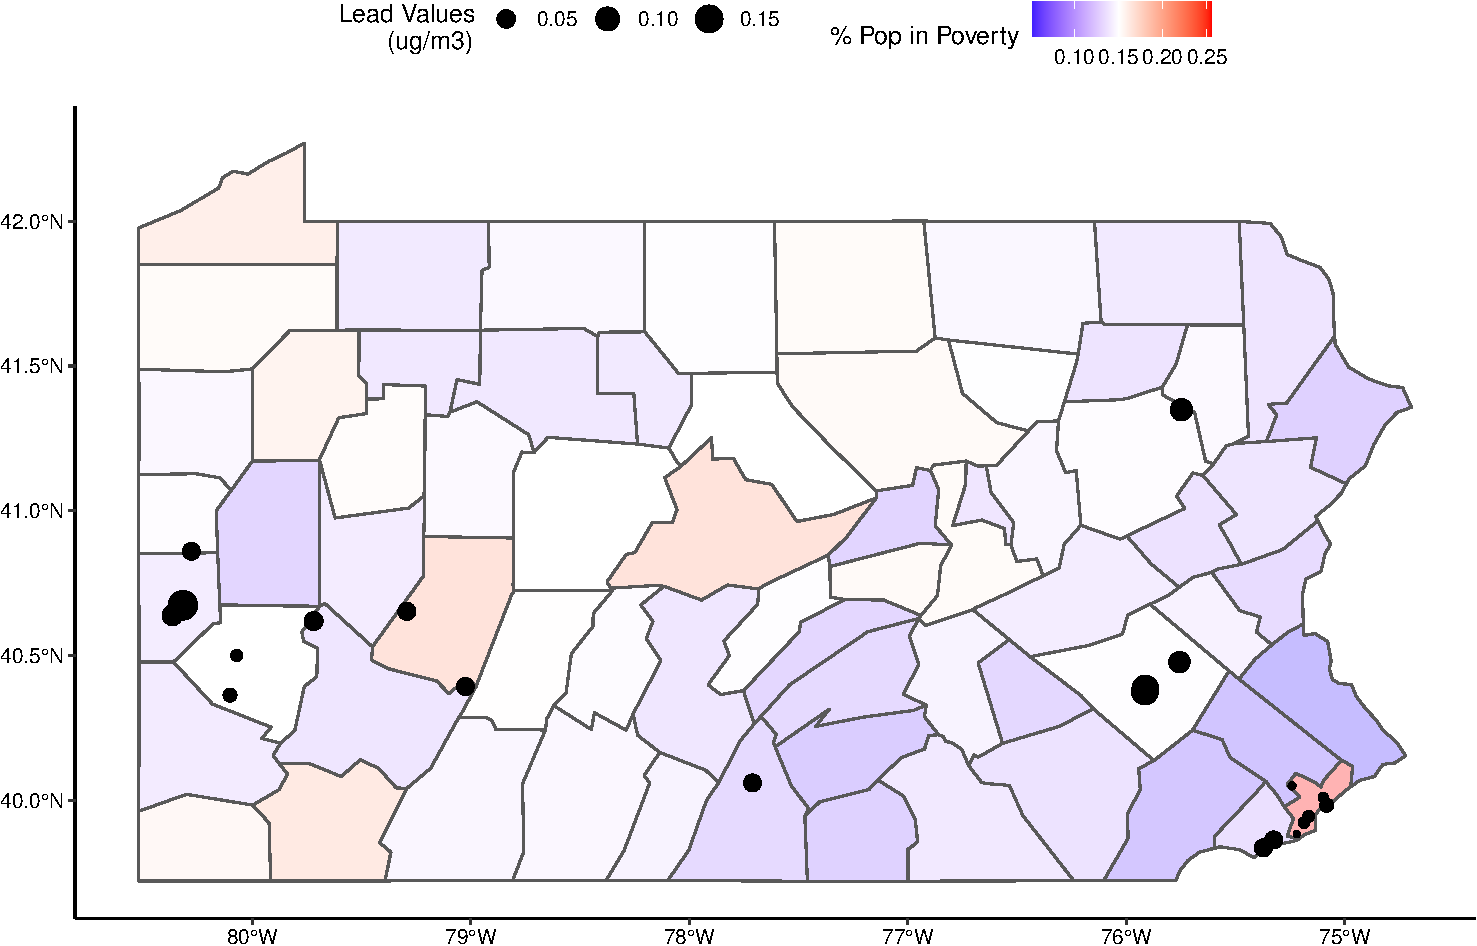
\includegraphics{Alcorn_Bao_Hermanson_ENV872_Project_files/figure-latex/spatial-analysis 2010-1} \hfill{}

\caption{2010 Mean Lead Levels Across Pennsylvania}\label{fig:spatial-analysis 2010}
\end{figure}

\begin{figure}

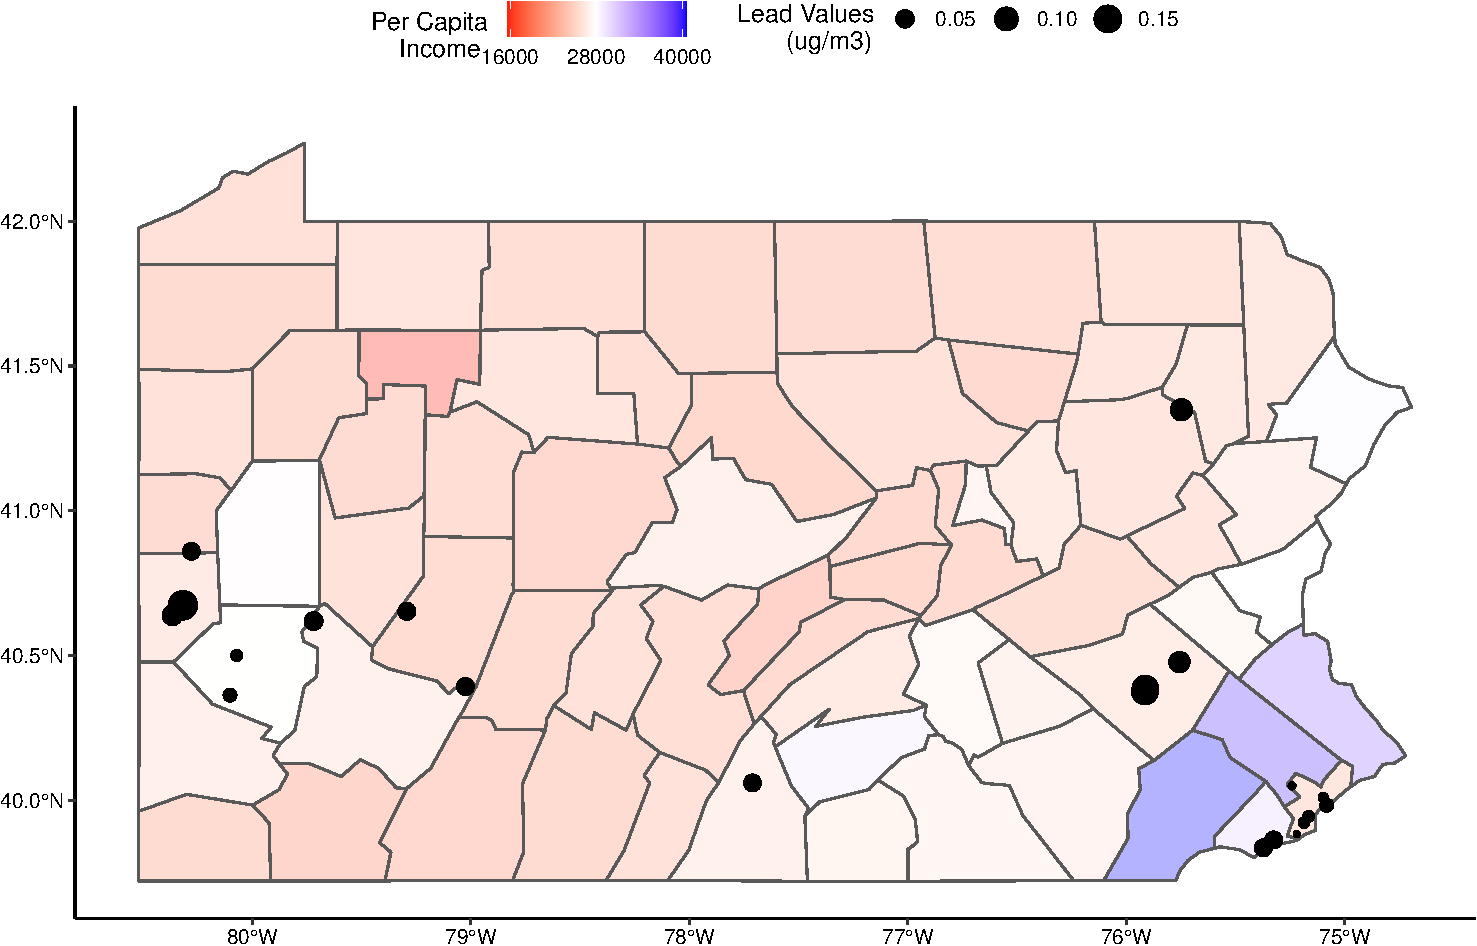
\includegraphics{Alcorn_Bao_Hermanson_ENV872_Project_files/figure-latex/spatial analysis 2010.2-1} \hfill{}

\caption{2010 Mean Lead Levels Across Pennsylvania}\label{fig:spatial analysis 2010.2}
\end{figure}

\begin{figure}

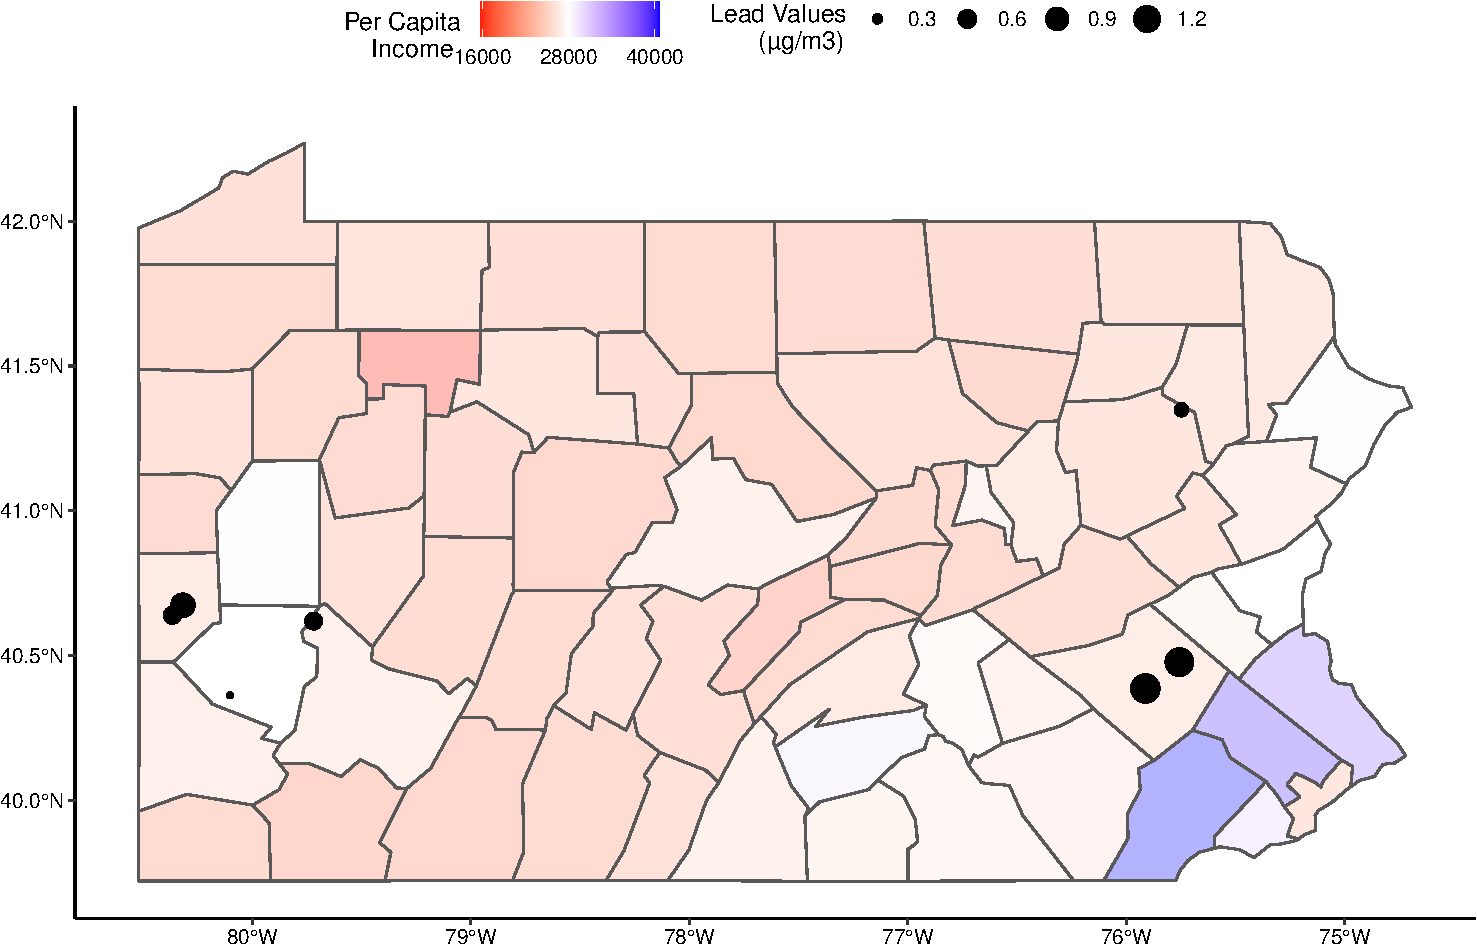
\includegraphics{Alcorn_Bao_Hermanson_ENV872_Project_files/figure-latex/spatial-analysis 2010.3-1} \hfill{}

\caption{2010 Max Lead Levels over .15 (µg/m3)}\label{fig:spatial-analysis 2010.3}
\end{figure}

\begin{verbatim}
## [1] 0.02118966 0.17580357
\end{verbatim}

\begin{figure}

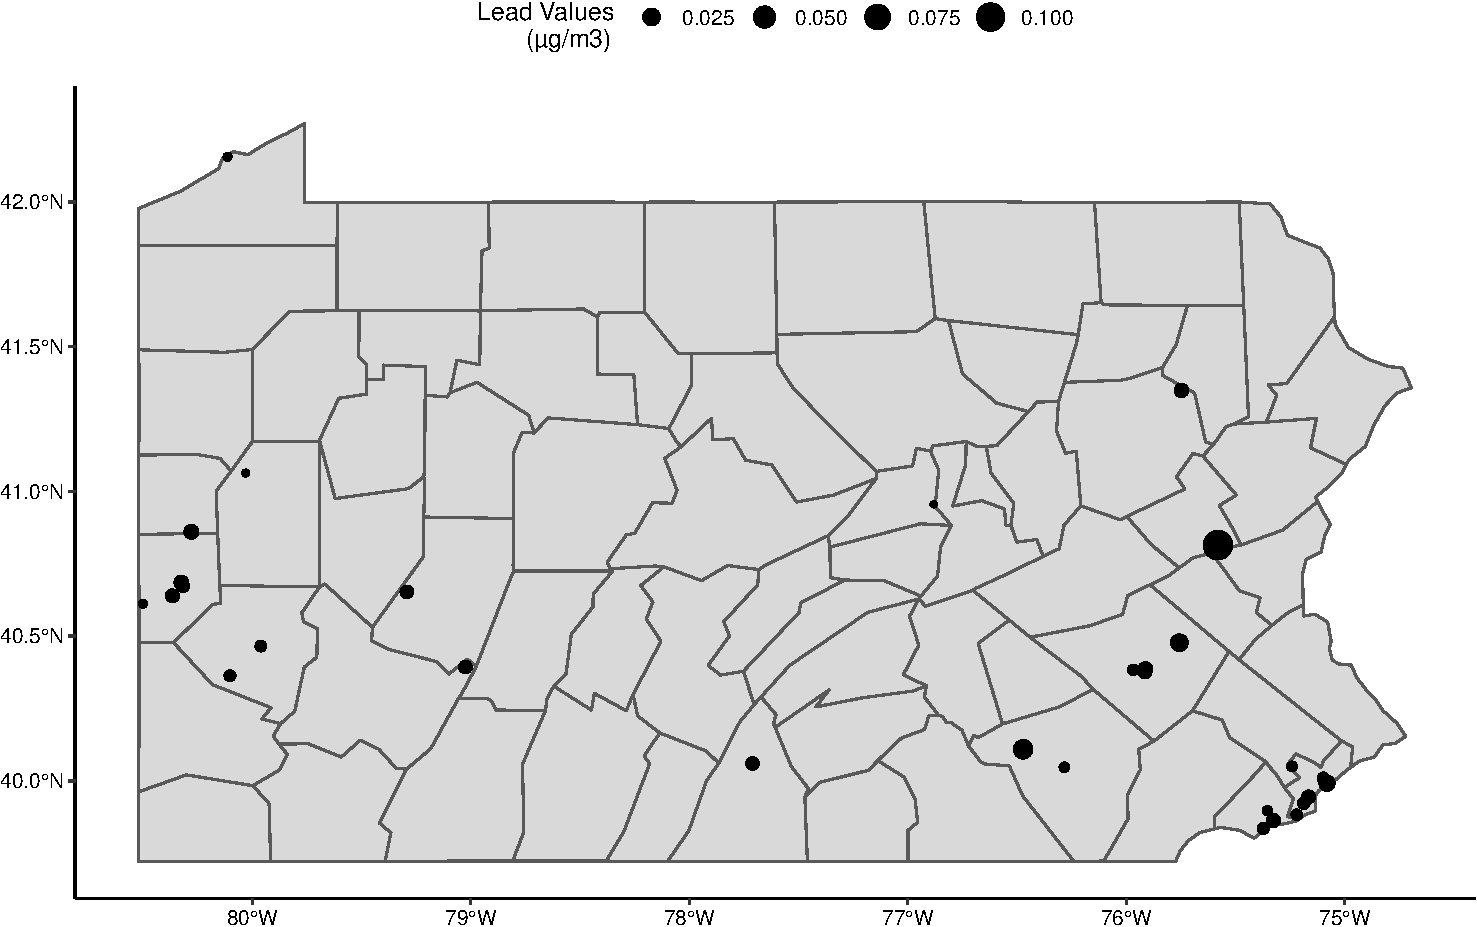
\includegraphics{Alcorn_Bao_Hermanson_ENV872_Project_files/figure-latex/spatial analysis 2015.4-1} \hfill{}

\caption{2015 Mean Lead Levels Across Pennsylvania}\label{fig:spatial analysis 2015.4}
\end{figure}

\begin{figure}
\centering
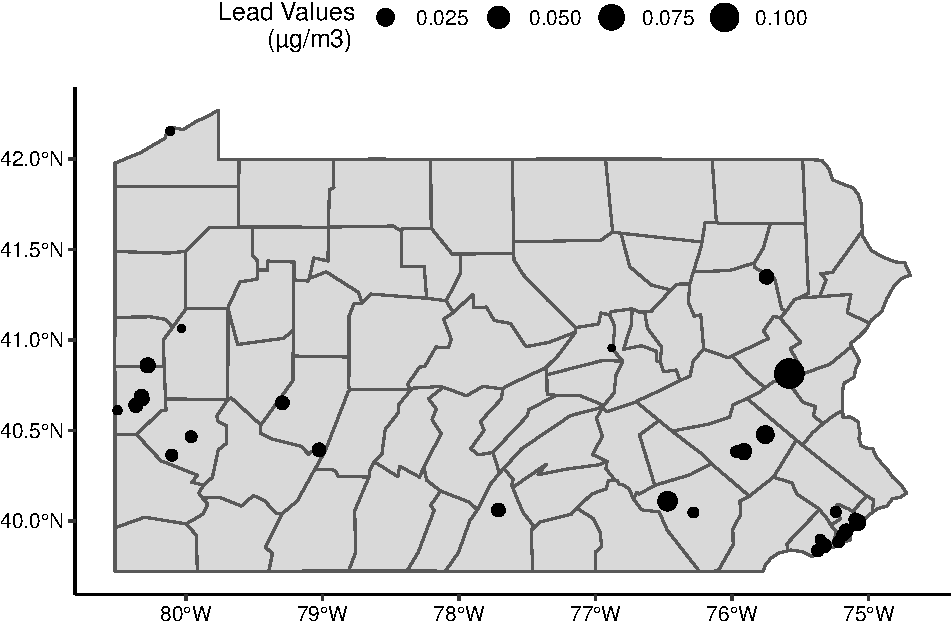
\includegraphics{Alcorn_Bao_Hermanson_ENV872_Project_files/figure-latex/spatial analysis 2015.5-1.pdf}
\caption{2015 Mean Lead Levels Across Pennsylvania}
\end{figure}

\begin{figure}
\centering
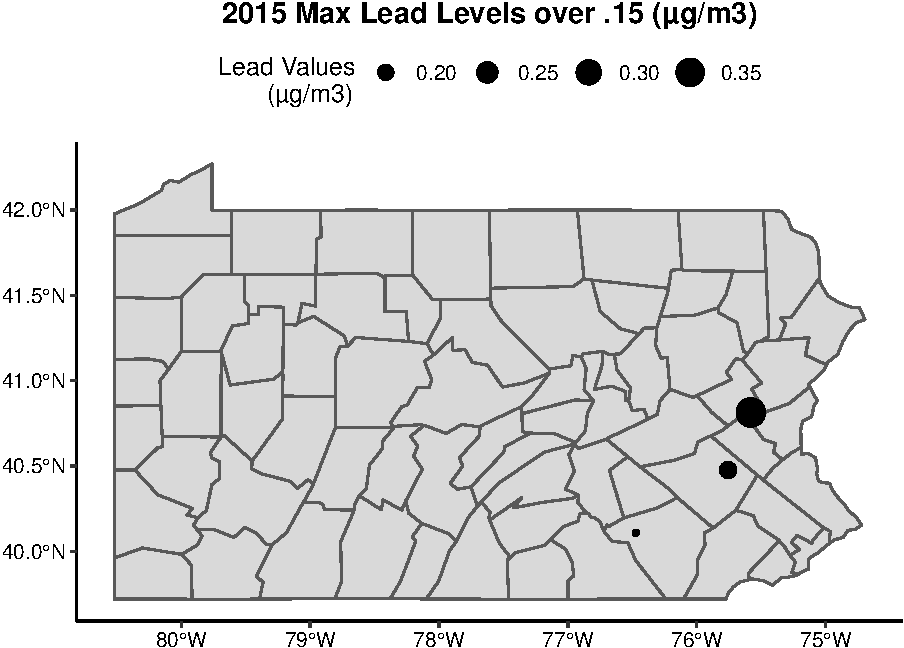
\includegraphics{Alcorn_Bao_Hermanson_ENV872_Project_files/figure-latex/spatial analysis 2015.6-1.pdf}
\caption{2015 Max Lead Levels over .15 (µg/m3)}
\end{figure}

\begin{figure}

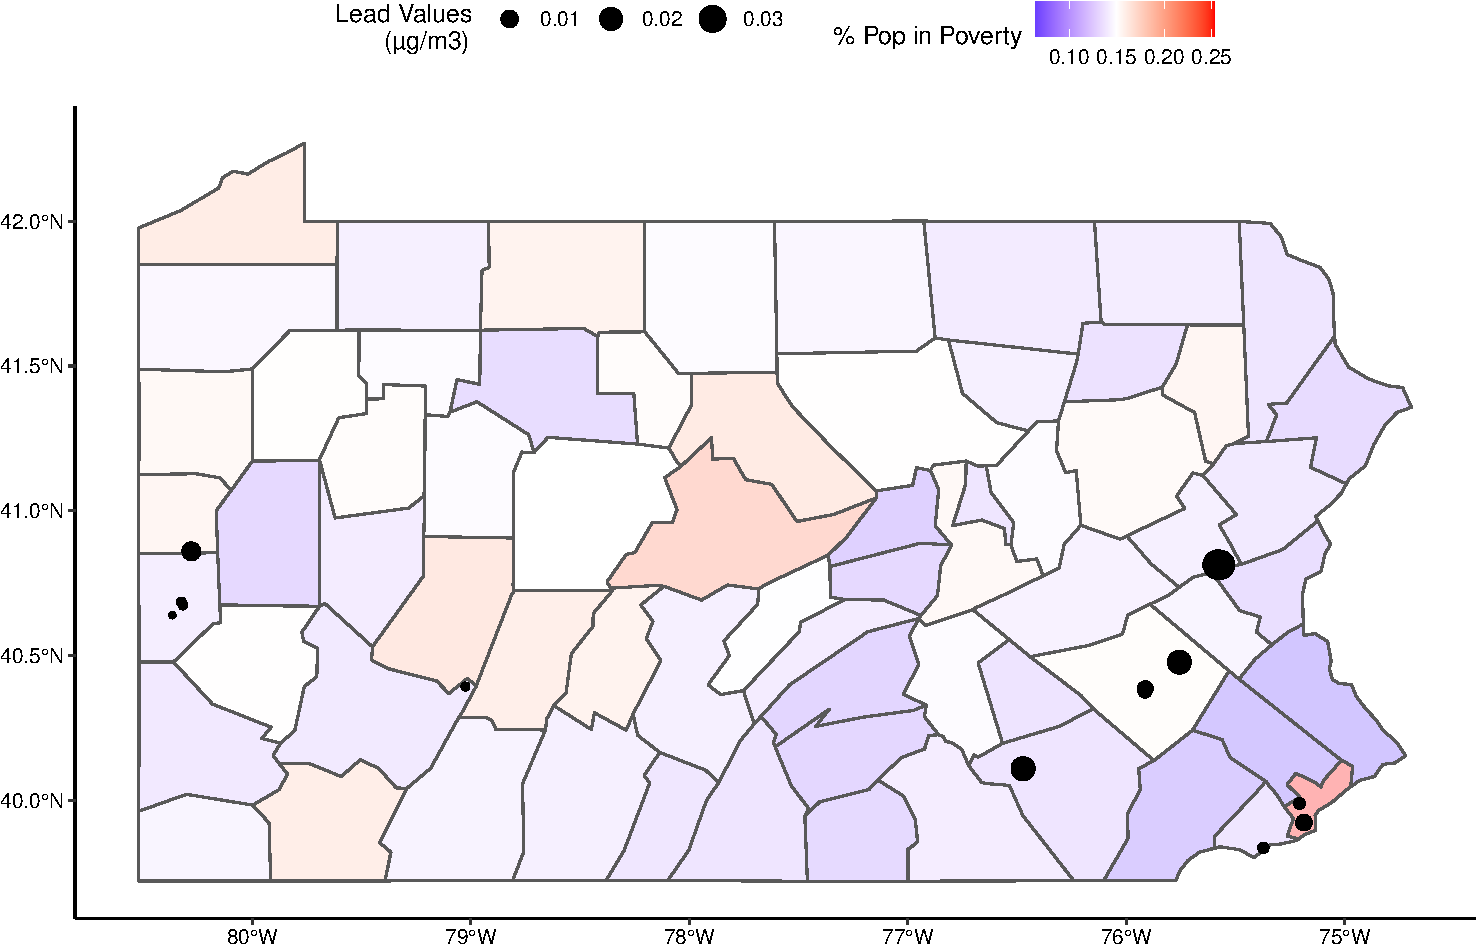
\includegraphics{Alcorn_Bao_Hermanson_ENV872_Project_files/figure-latex/spatial analysis 2020.1-1} \hfill{}

\caption{2020 Mean Lead Levels Across Pennsylvania}\label{fig:spatial analysis 2020.1}
\end{figure}

\begin{figure}

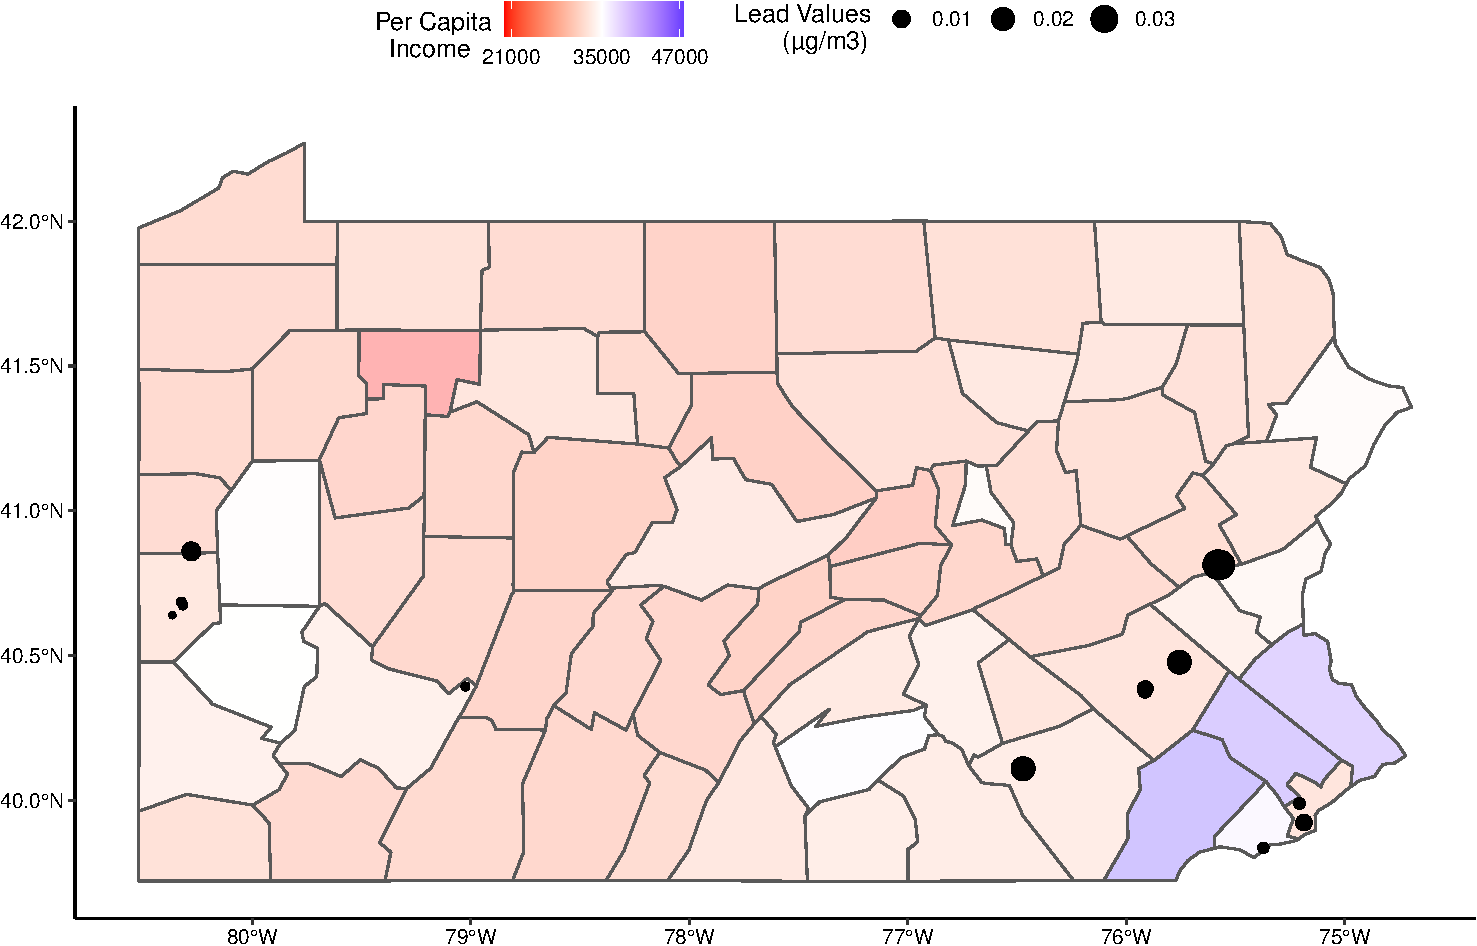
\includegraphics{Alcorn_Bao_Hermanson_ENV872_Project_files/figure-latex/spatial analysis 2020.2-1} \hfill{}

\caption{2020 Mean Lead Levels Across Pennsylvania}\label{fig:spatial analysis 2020.2}
\end{figure}

\begin{figure}

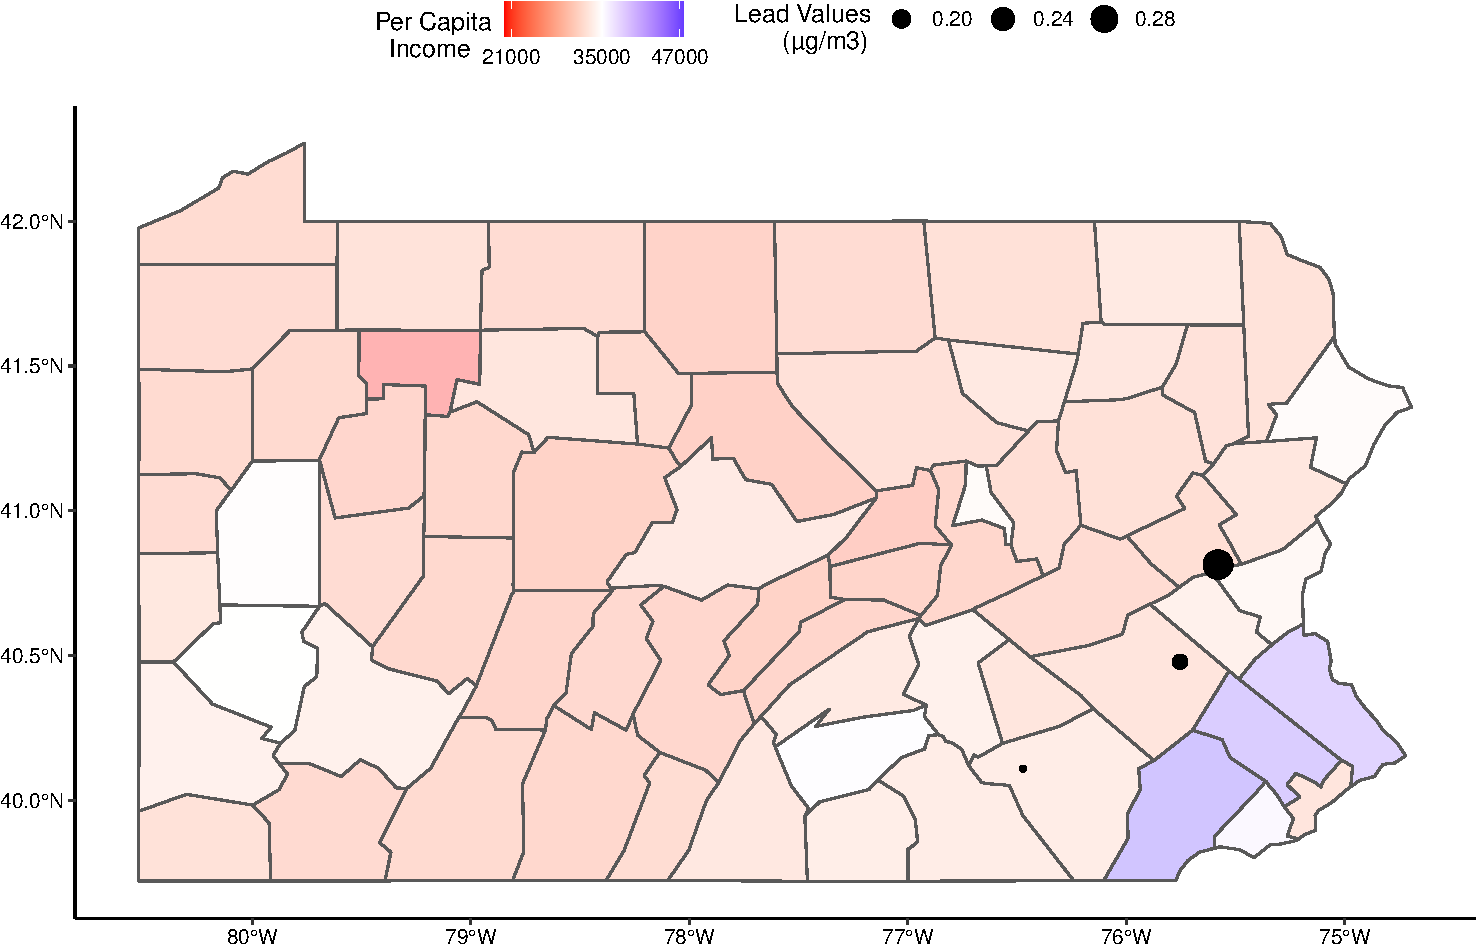
\includegraphics{Alcorn_Bao_Hermanson_ENV872_Project_files/figure-latex/spatial analysis 2020.3-1} \hfill{}

\caption{2020 Max Lead Levels over .15 (µg/m3)}\label{fig:spatial analysis 2020.3}
\end{figure}

\hypertarget{final-model-model-9}{%
\subsubsection{Final Model (Model 9)}\label{final-model-model-9}}

\hypertarget{blood-lead-beta1-x-log_metal-beta2-x-log_incinerate-beta4-x-meanpercapincome-beta5-x-pov2}{%
\paragraph{Blood lead = (beta1 x log\_metal) + (beta2 x log\_incinerate)
+ (beta4 x meanPerCapIncome) + (beta5 x
POV\$\^{}\$2)}\label{blood-lead-beta1-x-log_metal-beta2-x-log_incinerate-beta4-x-meanpercapincome-beta5-x-pov2}}

This model is statistically insignificant overall, with an f-statistics
p-value (0.29) being far greater than 0.05. The coefficient of meanPCI
(mean per-capita income) was statistically significant (p \textless{}
0.05), and can be interpreted as every decrease in income by 2,877
dollars is correlated with a 1\% increase in blood-lead levels in
children.

The low significance of this model is not surprising, given the
limitations of the data. The number of metal/incinerator plants may not
necessarily reflect the quantity of particulate lead being emitted,
which likely varies greatly between plants. If data were able to be
obtained about how much smoke/lead-particulate matter is being emitted
per plant, then that would have been more useful. The same applies to
airports; it is likely that the quantity of airports does not matter so
much as the number of flights and size of planes cycling through each
airport; were FAA data on these parameters available, they would have
been carried out. This is ultimately why the airport data was omitted
from the final model.

Quantity of plants/airports would have been more useful if the
geographic units used in this model were smaller -- county-level data
was the smallest data we could work with, given the reported blood lead
levels reported by the CDC were at a county level. Another geographical
consideration is that lead-emissions from the studied sources may not
affect their respective counties and instead disperse to other counties.

Of further concern with the metal processing data was that the range of
metal-processing plants was low across counties (max number of plants
was 12, min 0), with the mean being 1.72 plants/county. Such skewness of
the mean may not be appropriate for an OLS regression.

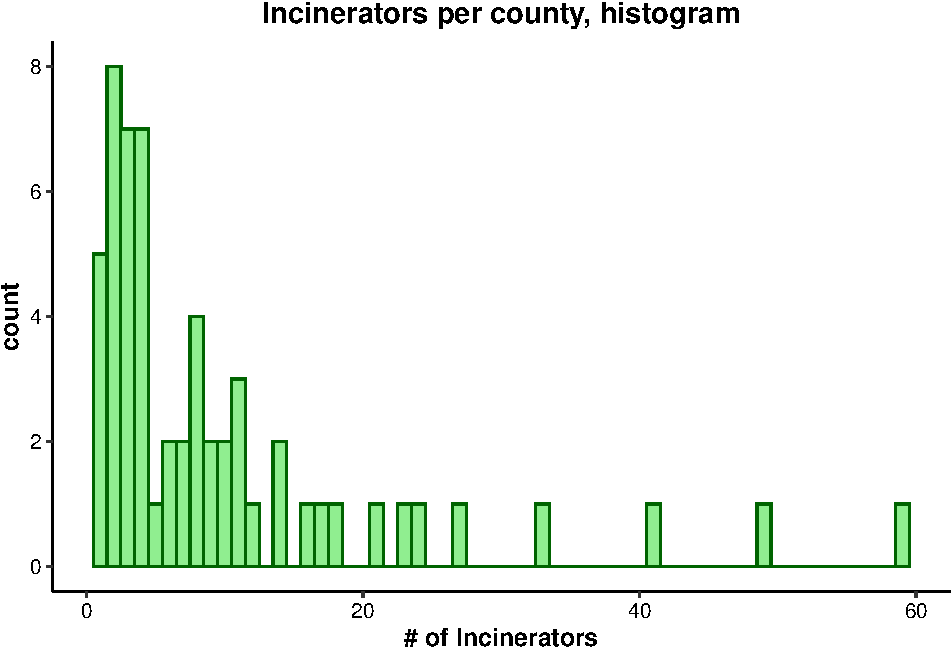
\includegraphics{Alcorn_Bao_Hermanson_ENV872_Project_files/figure-latex/setuping section-1.pdf}
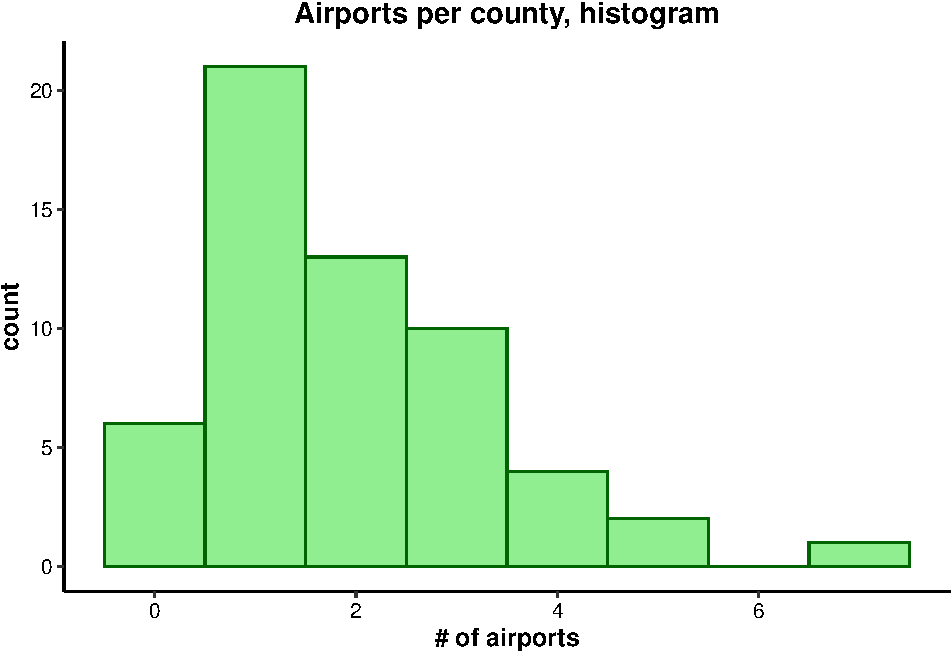
\includegraphics{Alcorn_Bao_Hermanson_ENV872_Project_files/figure-latex/setuping section-2.pdf}
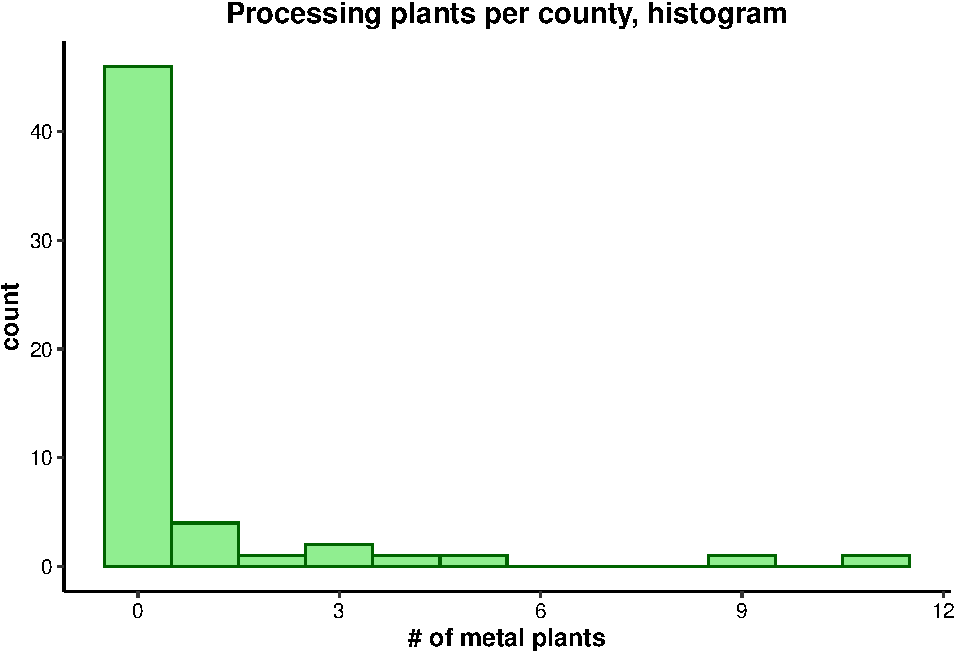
\includegraphics{Alcorn_Bao_Hermanson_ENV872_Project_files/figure-latex/setuping section-3.pdf}

\begin{table}[!h]

\caption{\label{tab:sum stats1}Metal Processing Summary Stats}
\centering
\begin{tabular}[t]{rrrrrr}
\toprule
Length & Mean & Median & Std\_Dev & Minimum & Maximum\\
\midrule
57 & 0.7192982 & 0 & 2.068077 & 0 & 11\\
\bottomrule
\end{tabular}
\end{table}
\begin{table}[!h]

\caption{\label{tab:sum stats2}Incinerator Summary Stats}
\centering
\begin{tabular}[t]{rrrrrr}
\toprule
Length & Mean & Median & Std\_Dev & Minimum & Maximum\\
\midrule
57 & 10.03509 & 6 & 11.93728 & 1 & 59\\
\bottomrule
\end{tabular}
\end{table}

\begin{table}[!h]

\caption{\label{tab:sum stats3}Airport Summary Stats}
\centering
\begin{tabular}[t]{rrrrrr}
\toprule
Length & Mean & Median & Std\_Dev & Minimum & Maximum\\
\midrule
57 & 1.929825 & 2 & 1.425027 & 0 & 7\\
\bottomrule
\end{tabular}
\end{table}

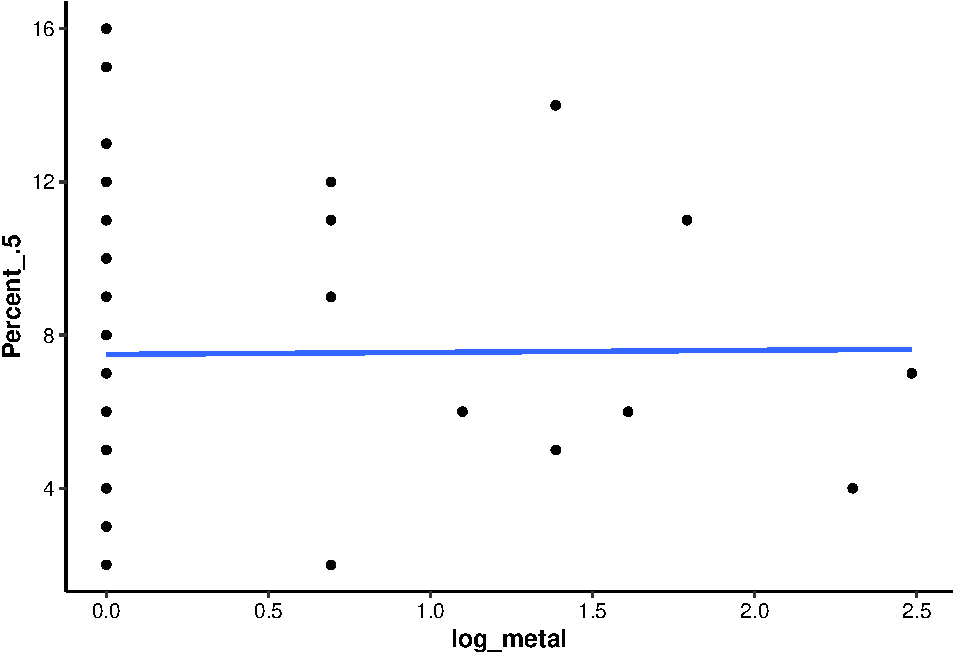
\includegraphics{Alcorn_Bao_Hermanson_ENV872_Project_files/figure-latex/linear plotssss -1.pdf}
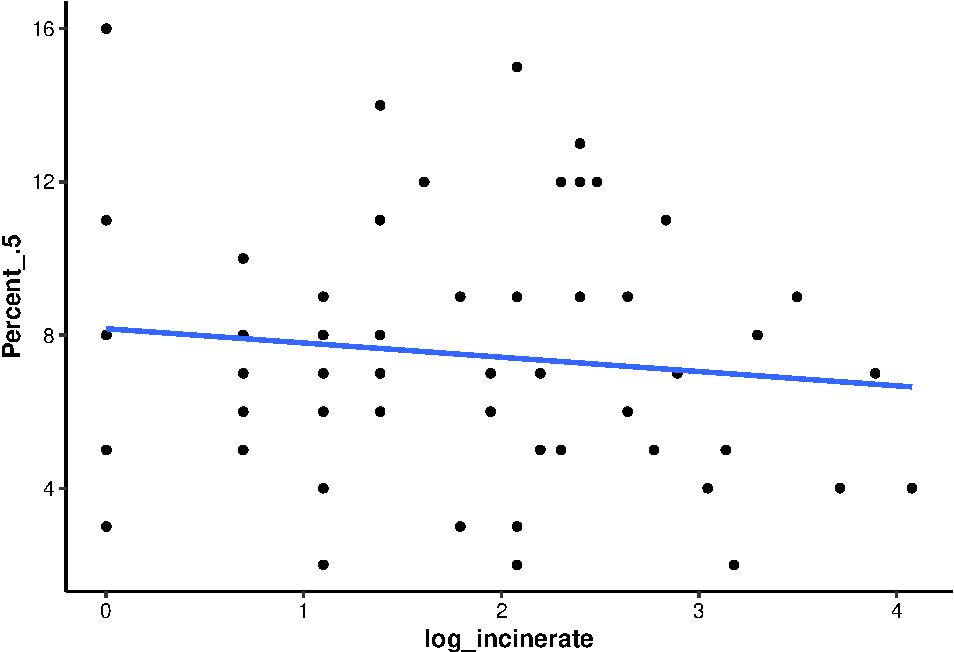
\includegraphics{Alcorn_Bao_Hermanson_ENV872_Project_files/figure-latex/linear plotssss -2.pdf}
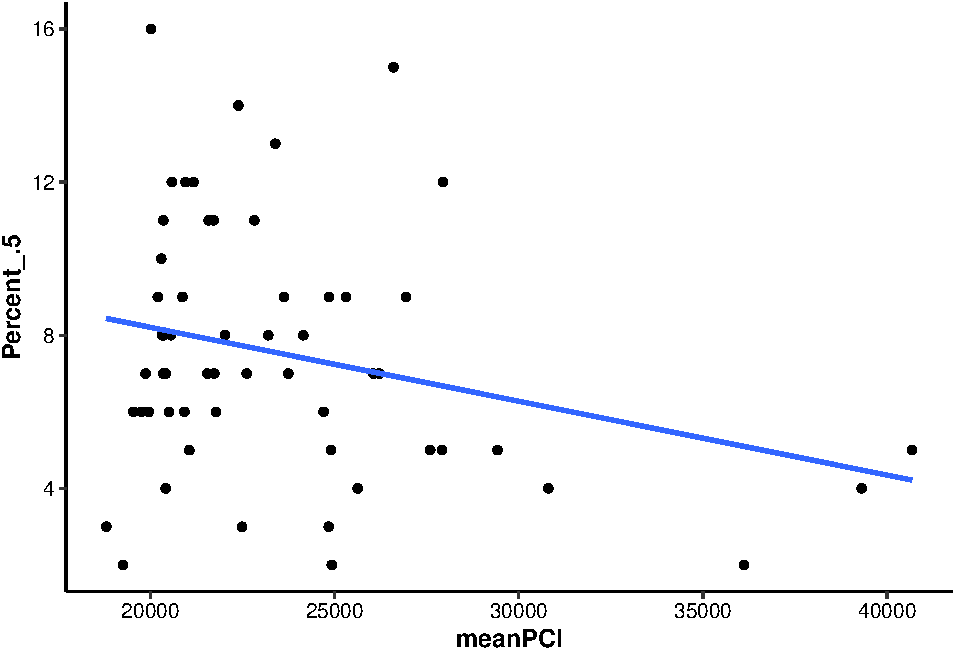
\includegraphics{Alcorn_Bao_Hermanson_ENV872_Project_files/figure-latex/linear plotssss -3.pdf}
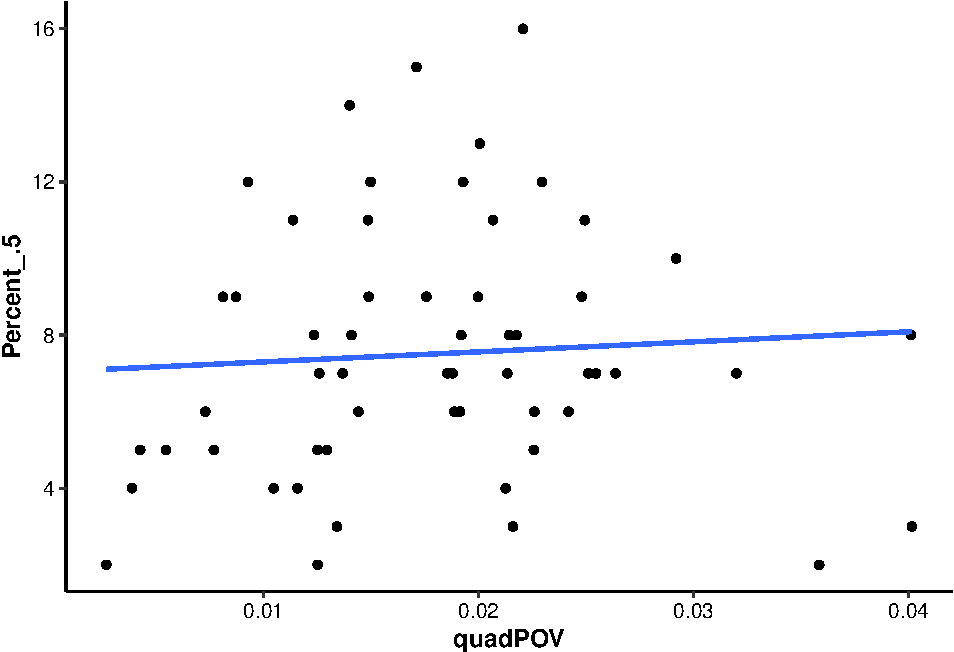
\includegraphics{Alcorn_Bao_Hermanson_ENV872_Project_files/figure-latex/linear plotssss -4.pdf}
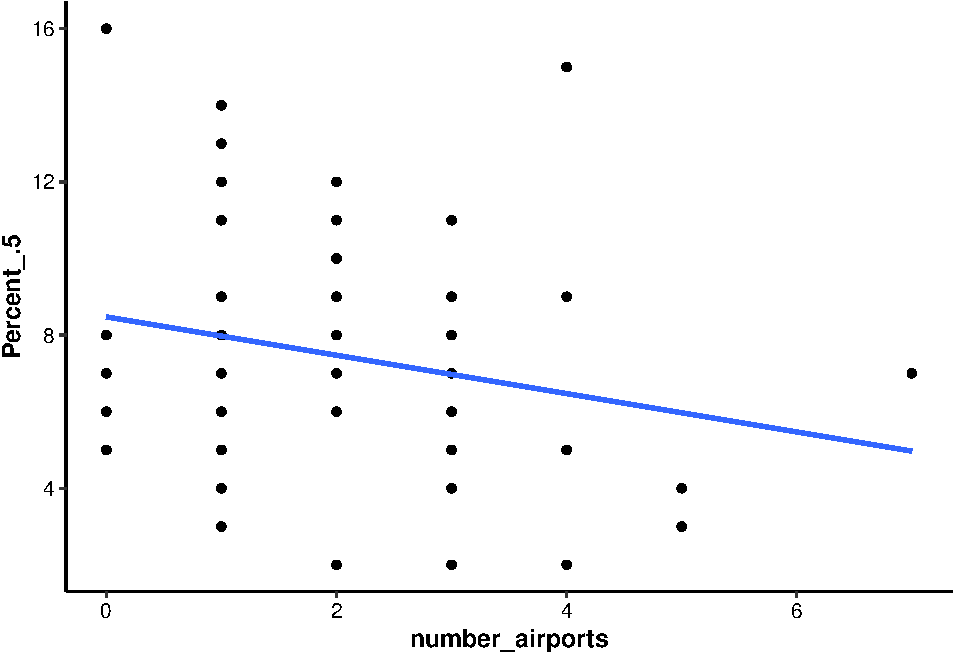
\includegraphics{Alcorn_Bao_Hermanson_ENV872_Project_files/figure-latex/linear plotssss -5.pdf}

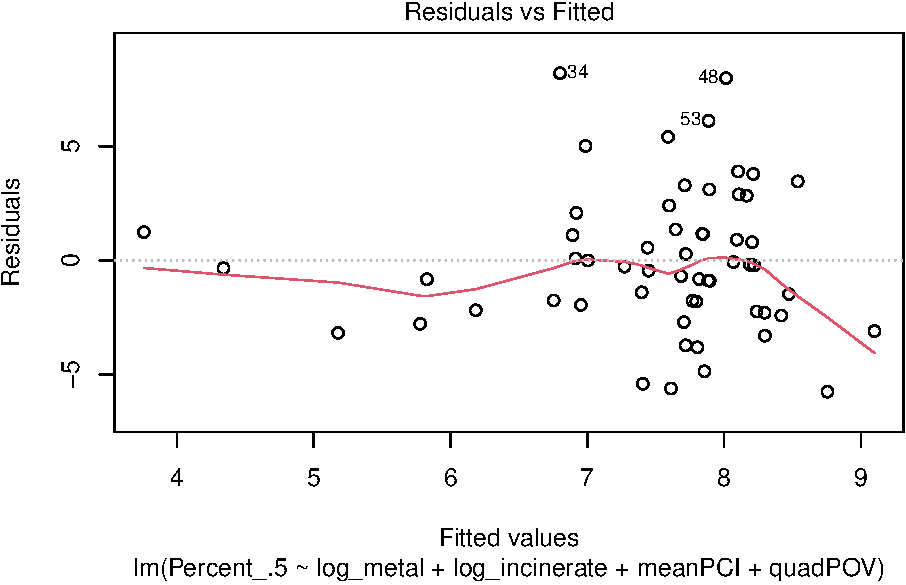
\includegraphics{Alcorn_Bao_Hermanson_ENV872_Project_files/figure-latex/analysis tools2-1.pdf}
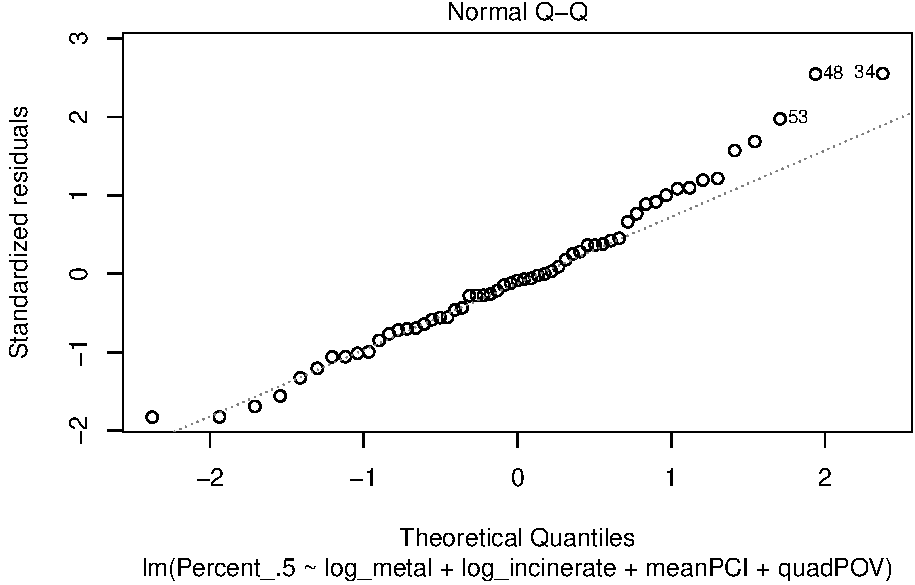
\includegraphics{Alcorn_Bao_Hermanson_ENV872_Project_files/figure-latex/analysis tools2-2.pdf}
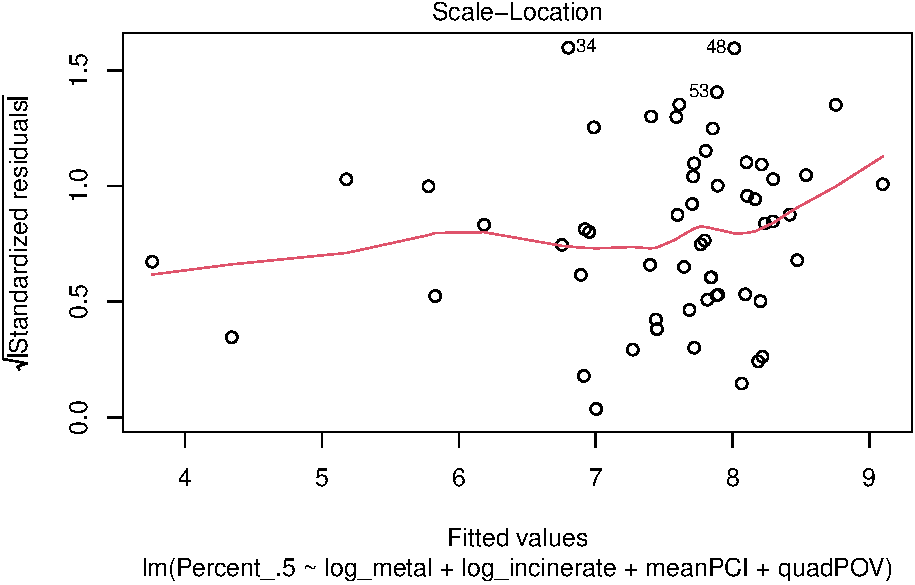
\includegraphics{Alcorn_Bao_Hermanson_ENV872_Project_files/figure-latex/analysis tools2-3.pdf}
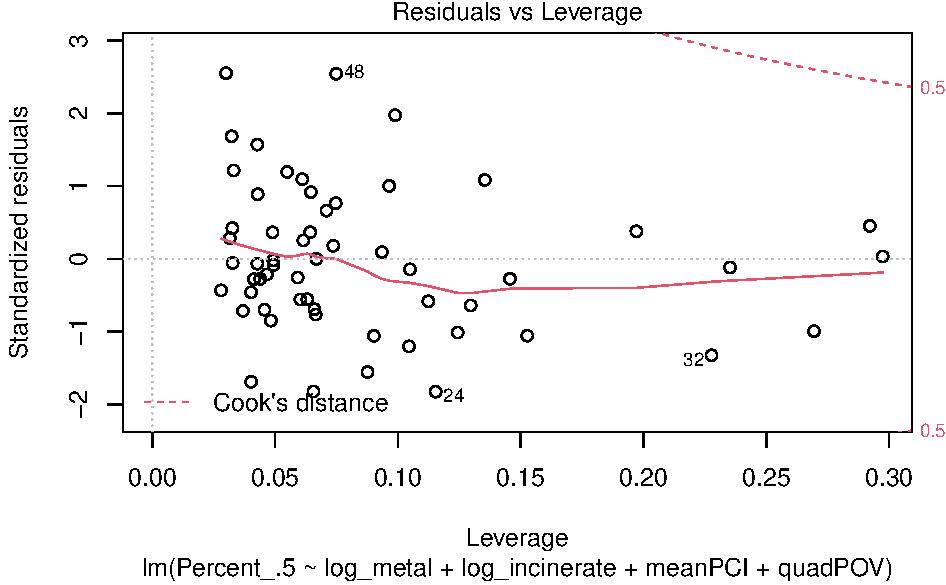
\includegraphics{Alcorn_Bao_Hermanson_ENV872_Project_files/figure-latex/analysis tools2-4.pdf}

\begin{figure}

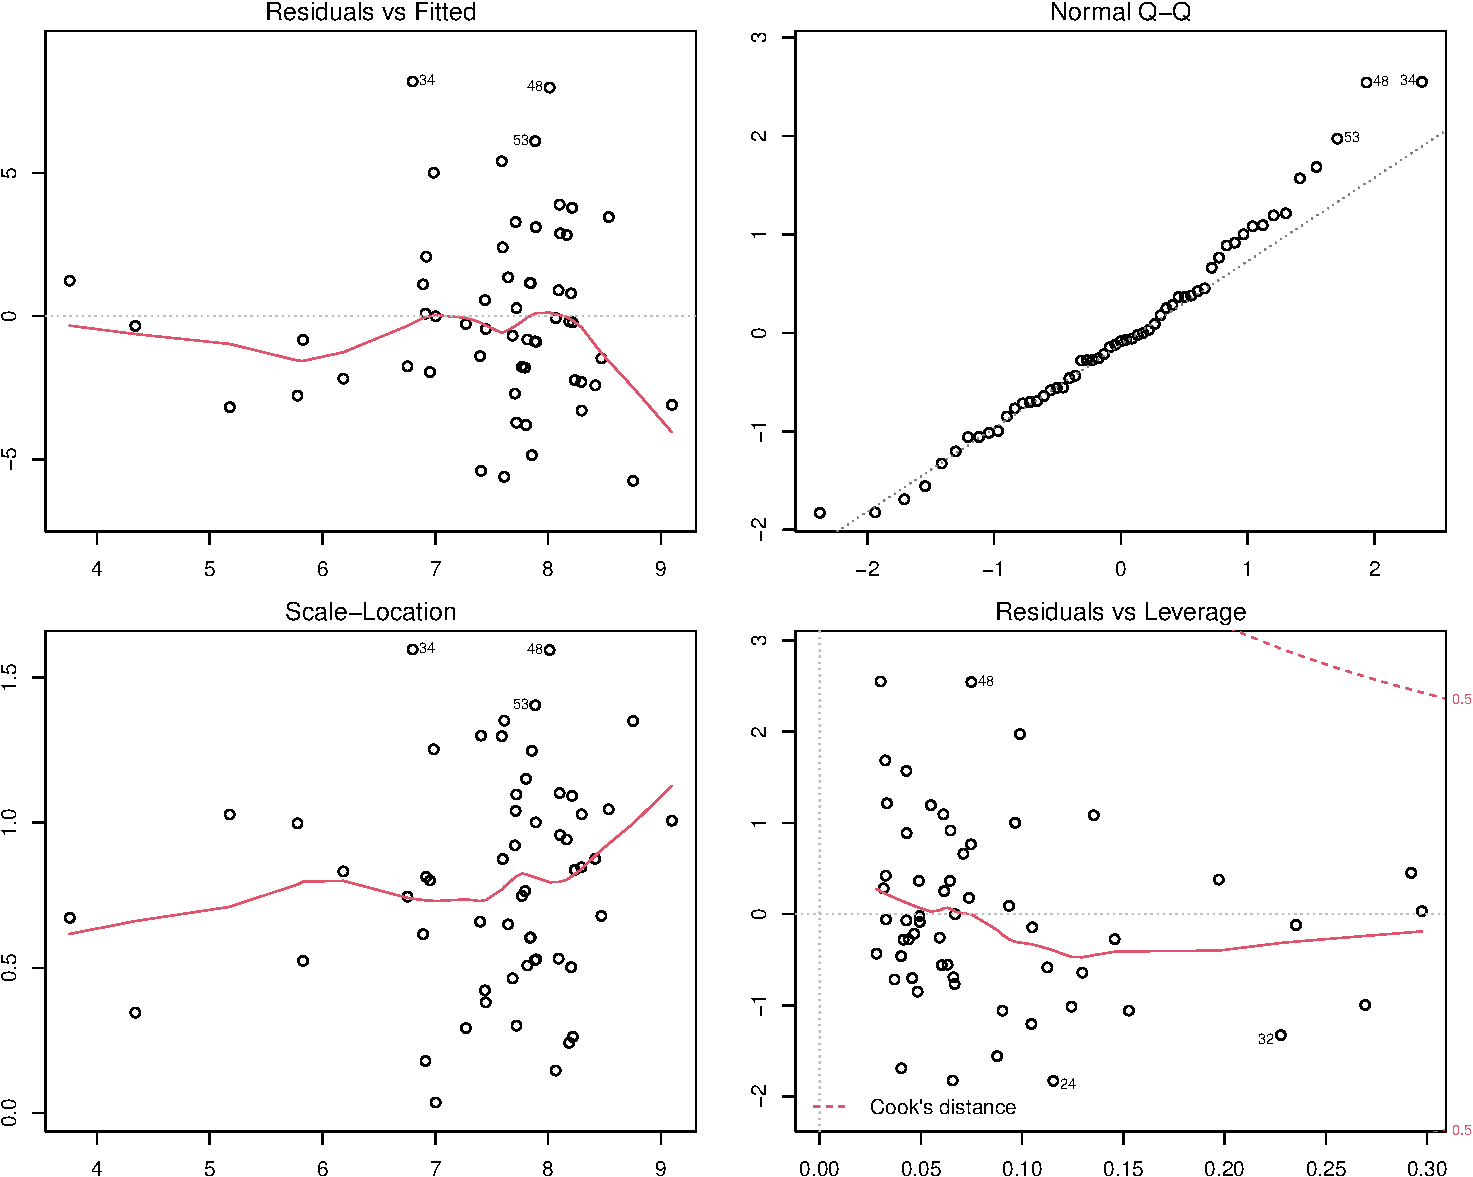
\includegraphics{Alcorn_Bao_Hermanson_ENV872_Project_files/figure-latex/analyis final-1} \hfill{}

\caption{Model Assumption Plots}\label{fig:analyis final}
\end{figure}

\begin{verbatim}
## 
## Call:
## lm(formula = Percent_.5 ~ log_metal + log_incinerate + meanPCI + 
##     quadPOV, data = i_a_m_b_join)
## 
## Residuals:
##     Min      1Q  Median      3Q     Max 
## -5.7545 -2.1846 -0.2716  1.3546  8.2000 
## 
## Coefficients:
##                  Estimate Std. Error t value Pr(>|t|)    
## (Intercept)     1.519e+01  3.865e+00   3.929 0.000253 ***
## log_metal      -1.463e-01  7.386e-01  -0.198 0.843749    
## log_incinerate  1.749e-01  4.964e-01   0.352 0.725962    
## meanPCI        -2.877e-04  1.403e-04  -2.051 0.045363 *  
## quadPOV        -6.406e+01  6.798e+01  -0.942 0.350397    
## ---
## Signif. codes:  0 '***' 0.001 '**' 0.01 '*' 0.05 '.' 0.1 ' ' 1
## 
## Residual standard error: 3.264 on 52 degrees of freedom
## Multiple R-squared:  0.08933,    Adjusted R-squared:  0.01928 
## F-statistic: 1.275 on 4 and 52 DF,  p-value: 0.2917
\end{verbatim}

\begin{verbatim}
## [1] 303.3744
\end{verbatim}

\begin{verbatim}
##      log_metal log_incinerate        meanPCI        quadPOV 
##       1.044164       1.422348       2.158539       1.639418
\end{verbatim}

\begin{verbatim}
## number_metal_plants number_incinerators     number_airports             meanPCI 
##            1.053063            2.118427            1.871259            2.954335 
##             meanPOV 
##            2.189966
\end{verbatim}

\newpage

\hypertarget{summary-and-conclusions}{%
\section{Summary and Conclusions}\label{summary-and-conclusions}}

We found that four of the five most populous metropolitan areas
Philadelphia-Camden-Wilmington, PA-NJ-DE-MD (2010-2020), Pittsburgh, PA
(2010-2020), Allentown-Bethlehem-Easton, PA-NJ (2012-2020), and
Scranton--Wilkes-Barre--Hazleton, PA (2010-2018) in Pennsylvania had
downward monotonic trends for daily and monthly mean air lead
concentrations (p\textless0.05). The Lancaster, PA metropolitan area did
not show a monotonic downward trend for air lead levels, which may be
attributed to other factors not explored in this study such as
industrial emissions between 2012 and 2020. It is important to note that
the downward trend for the other four metropolitan areas may be
attributed to the banning of lead in paints in 1978, the banning of lead
in vehicle fuels in 1996, the waning of lead-smelting industry, or other
factors such as lead abatement programs from 2010 to 2020 in
Pennsylvania into the twenty-first century (Schwarz et al., 2012).
Future studies may look at conducting multiple linear regression to
assess air lead levels in association with remediation measures to
reduce air lead exposure or other factors such as climate factors like
temperature and wind speed, which may influence quantity of lead in
ambient air (Kinney, 2018). Obtaining census-block specific data and air
emissions data will enable stronger multilinear regression in future
models.

\newpage

\hypertarget{references}{%
\section{References}\label{references}}

Ab Latif Wani, A. A., \& Usmani, J. A. (2015). Lead toxicity: a review.
Interdisciplinary toxicology, 8(2), 55. doi: 10.1515/intox-2015-0009

About Air Data Reports. (2021). United States Environmental Protection
Agency. Retrieved from
\href{https://www.epa.gov/outdoor-air-quality-data/about-air-data-reports}{link}

American Lung Association (2021). Most Polluted Cities. Retrieved from
\href{https://www.lung.org/research/sota/city-rankings/most-polluted-cities}{link}

CDC Social Vulnerability Index Data {[}internet database{]} available
via
\href{https://www.atsdr.cdc.gov/placeandhealth/svi/data_documentation_download.html}{link}

Kinney, P. L. (2018). Interactions of climate change, air pollution, and
human health. Current environmental health reports, 5(1), 179-186.
\href{https://doi.org/10.1007/s40572-018-0188-x}{link}

O'Shea, M. J., Vann, D. R., Hwang, W. T., \& Gieré, R. (2020). A
mineralogical and chemical investigation of road dust in Philadelphia,
PA, USA. Environmental Science and Pollution Research, 1-20.
\href{https://doi.org/10.1007/s11356-019-06746-y}{link}

PA Department of Health (2014). 2014 Childhood Lead Surveillance Annual
Report. Retrieved from
\href{https://www.health.pa.gov/topics/Documents/Environmental\%20Health/2014\%20Lead\%20Surveillance\%20Annual\%20Report.pdf}{link}

Pizzol, M., Thomsen, M., \& Andersen, M. S. (2010). Long-term human
exposure to lead from different media and intake pathways. Science of
the total environment, 408(22), 5478-5488.
\href{https://doi.org/10.1016/j.scitotenv.2010.07.077}{link}

Schwarz, K., Pickett, S. T., Lathrop, R. G., Weathers, K. C., Pouyat, R.
V., \& Cadenasso, M. L. (2012). The effects of the urban built
environment on the spatial distribution of lead in residential soils.
Environmental pollution, 163, 32-39.
\href{https://doi.org/10.1016/j.envpol.2011.12.003}{link}

Stevens, S. K. (1955). A Century of Industry in Pennsylvania.
Pennsylvania History: A Journal of Mid-Atlantic Studies, 22(1), 49-68.

United Health Foundation. (2019). America's Health Rankings. Retrieved
from
\href{https://assets.americashealthrankings.org/app/uploads/ahr_2019annualreport.pdf}{link}

US Census Bureau. (2019). Metropolitan and Micropolitan Statistical Area
Population Estimates and Estimated Components of Change: April 1, 2010
to July 1, 2019 (CBSA-EST2019-alldata). Retrieved from
\href{https://www.census.gov/data/tables/time-series/demo/popest/2010s-total-metro-and-micro-statistical-areas.html\#par_textimage}{link}

US Census Bureau. (2020a). CBSA-EST2019-alldata: Annual Resident
Population Estimates and Estimated Components of Resident Population
Change for Metropolitan and Micropolitan Statistical Areas and Their
Geographic Components: April 1, 2010 to July 1, 2019
\href{https://www2.census.gov/programs-surveys/popest/technical-documentation/file-layouts/2010-2019/cbsa-est2019-alldata.pdf}{link}

US Census Bureau (2020b). METHODOLOGY FOR THE UNITED STATES POPULATION
ESTIMATES: VINTAGE 2019 Nation, States, Counties, and Puerto Rico --
April 1, 2010 to July 1, 2019. Retrieved from
\href{https://www2.census.gov/programs-surveys/popest/technical-documentation/methodology/2010-2019/natstcopr-methv2.pdf}{link}

US Environmental Protection Agency. Air Quality System Data Mart
{[}internet database{]} available via
\href{https://www.epa.gov/airdata.\%20Accessed\%20April\%2005,\%202021.}{link}

US EPA. (2021a). Basic Information about Lead Air Pollution. Lead Air
Pollution. Retrieved from
\href{https://www.epa.gov/lead-air-pollution/basic-information-about-lead-air-pollution\#:~:text=At\%20the\%20national\%20level\%2C\%20major,usually\%20found\%20near\%20lead\%20smelters.}{link}

US EPA. (2021b). Timeline of Lead (Pb) National Ambient Air Quality
Standards (NAAQS) Retrieved from
\href{https://www.epa.gov/lead-air-pollution/timeline-lead-pb-national-ambient-air-quality-standards-naaqs}{link}

WHO. (2021). Lead poisoning and health. Retrieved April 24, 2021, from
\href{https://www.who.int/news-room/fact-sheets/detail/lead-poisoning-and-health}{link}

\end{document}
